
%% bare_conf.tex
%% V1.3
%% 2007/01/11
%% by Michael Shell
%% See:
%% http://www.michaelshell.org/
%% for current contact information.
%%
%% This is a skeleton file demonstrating the use of IEEEtran.cls
%% (requires IEEEtran.cls version 1.7 or later) with an IEEE conference paper.
%%
%% Support sites:
%% http://www.michaelshell.org/tex/ieeetran/
%% http://www.ctan.org/tex-archive/macros/latex/contrib/IEEEtran/
%% and
%% http://www.ieee.org/

%%*************************************************************************
%% Legal Notice:
%% This code is offered as-is without any warranty either expressed or
%% implied; without even the implied warranty of MERCHANTABILITY or
%% FITNESS FOR A PARTICULAR PURPOSE! 
%% User assumes all risk.
%% In no event shall IEEE or any contributor to this code be liable for
%% any damages or losses, including, but not limited to, incidental,
%% consequential, or any other damages, resulting from the use or misuse
%% of any information contained here.
%%
%% All comments are the opinions of their respective authors and are not
%% necessarily endorsed by the IEEE.
%%
%% This work is distributed under the LaTeX Project Public License (LPPL)
%% ( http://www.latex-project.org/ ) version 1.3, and may be freely used,
%% distributed and modified. A copy of the LPPL, version 1.3, is included
%% in the base LaTeX documentation of all distributions of LaTeX released
%% 2003/12/01 or later.
%% Retain all contribution notices and credits.
%% ** Modified files should be clearly indicated as such, including  **
%% ** renaming them and changing author support contact information. **
%%
%% File list of work: IEEEtran.cls, IEEEtran_HOWTO.pdf, bare_adv.tex,
%%                    bare_conf.tex, bare_jrnl.tex, bare_jrnl_compsoc.tex
%%*************************************************************************

% *** Authors should verify (and, if needed, correct) their LaTeX system  ***
% *** with the testflow diagnostic prior to trusting their LaTeX platform ***
% *** with production work. IEEE's font choices can trigger bugs that do  ***
% *** not appear when using other class files.                            ***
% The testflow support page is at:
% http://www.michaelshell.org/tex/testflow/



% Note that the a4paper option is mainly intended so that authors in
% countries using A4 can easily print to A4 and see how their papers will
% look in print - the typesetting of the document will not typically be
% affected with changes in paper size (but the bottom and side margins will).
% Use the testflow package mentioned above to verify correct handling of
% both paper sizes by the user's LaTeX system.
%
% Also note that the "draftcls" or "draftclsnofoot", not "draft", option
% should be used if it is desired that the figures are to be displayed in
% draft mode.
%
\documentclass[conference]{IEEEtran}
% Add the compsoc option for Computer Society conferences.
%
% If IEEEtran.cls has not been installed into the LaTeX system files,
% manually specify the path to it like:
% \documentclass[conference]{../sty/IEEEtran}


% use Times
\usepackage{times}
% For figures
\usepackage{graphicx} % more modern
%\usepackage{epsfig} % less modern
\usepackage{subfigure} 
%\usepackage{caption}
%\usepackage{subcaption}

\usepackage{amsmath}
\usepackage{url}
\usepackage{verbatim}

% For citations
\usepackage{natbib}

% For algorithms
\usepackage{algorithm}
\usepackage{algorithmic}

\usepackage{array}
\newcolumntype{L}{>{\centering\arraybackslash}m{4.5cm}}
\newcolumntype{C}{>{\centering\arraybackslash}m{6.5cm}}
\usepackage{lipsum}

% As of 2011, we use the hyperref package to produce hyperlinks in the
% resulting PDF.  If this breaks your system, please commend out the
% following usepackage line and replace \usepackage{icml2015} with
% \usepackage[nohyperref]{icml2015} above.
\usepackage{hyperref}

\DeclareMathOperator{\x}{\mathbf{x}}
\DeclareMathOperator{\e}{\mathbf{e}}
\DeclareMathOperator{\M}{\mathbf{M}}
\DeclareMathOperator{\w}{\mathbf{w}}
\newcommand{\fix}{\marginpar{FIX}}
\newcommand{\new}{\marginpar{NEW}}
\edef\polishl{\l} 



\RequirePackage{latexsym}
\RequirePackage{amsmath}
\RequirePackage{amssymb} 
\RequirePackage{color} 
\RequirePackage{bm}
\RequirePackage{color}
\RequirePackage{picinpar}

%%%%%%%% Stock standard definitions %%%%%%%%%%%%%%%

\newcommand{\wbt}{\widetilde{\mathbf{w}}}
\DeclareMathOperator{\ab}{\mathbf{a}}
\DeclareMathOperator{\abh}{\widehat{\ab}}
\DeclareMathOperator{\bb}{\mathbf{b}}
\DeclareMathOperator{\bbh}{\widehat{\bb}}
\DeclareMathOperator{\cb}{\mathbf{c}}
\DeclareMathOperator{\db}{\mathbf{d}}
\DeclareMathOperator{\eb}{\mathbf{e}}
\DeclareMathOperator{\fb}{\mathbf{f}}
\DeclareMathOperator{\gb}{\mathbf{g}}
\DeclareMathOperator{\hb}{\mathbf{h}}
\DeclareMathOperator{\ib}{\mathbf{i}}
\DeclareMathOperator{\jb}{\mathbf{j}}
\DeclareMathOperator{\kb}{\mathbf{k}}
\DeclareMathOperator{\lb}{\mathbf{l}}
\DeclareMathOperator{\mb}{\mathbf{m}}
\DeclareMathOperator{\nbb}{\mathbf{n}}
\DeclareMathOperator{\ob}{\mathbf{o}}
\DeclareMathOperator{\pb}{\mathbf{p}}
\DeclareMathOperator{\qb}{\mathbf{q}}
\DeclareMathOperator{\rb}{\mathbf{r}}
\DeclareMathOperator{\sbb}{\mathbf{s}}
\DeclareMathOperator{\tb}{\mathbf{t}}
\DeclareMathOperator{\ub}{\mathbf{u}}
\DeclareMathOperator{\vb}{\mathbf{v}}
\DeclareMathOperator{\wb}{\mathbf{w}}
\DeclareMathOperator{\xb}{\mathbf{x}}
\DeclareMathOperator{\yb}{\mathbf{y}}
\DeclareMathOperator{\zb}{\mathbf{z}}
\renewcommand{\l}{\ell}

\DeclareMathOperator{\atilde}{\tilde{\ab}}
\DeclareMathOperator{\btilde}{\tilde{\bb}}
\DeclareMathOperator{\ctilde}{\tilde{\cb}}
\DeclareMathOperator{\dtilde}{\tilde{\db}}
\DeclareMathOperator{\etilde}{\tilde{\eb}}
\DeclareMathOperator{\ftilde}{\tilde{\fb}}
\DeclareMathOperator{\gtilde}{\tilde{\gb}}
\DeclareMathOperator{\htilde}{\tilde{\hb}}
\DeclareMathOperator{\itilde}{\tilde{\ib}}
\DeclareMathOperator{\jtilde}{\tilde{\jb}}
\DeclareMathOperator{\ktilde}{\tilde{\kb}}
\DeclareMathOperator{\ltilde}{\tilde{\lb}}
\DeclareMathOperator{\mtilde}{\tilde{\mb}}
\DeclareMathOperator{\ntilde}{\tilde{\nbb}}
\DeclareMathOperator{\otilde}{\tilde{\ob}}
\DeclareMathOperator{\ptilde}{\tilde{\pb}}
\DeclareMathOperator{\qtilde}{\tilde{\qb}}
\DeclareMathOperator{\rtilde}{\tilde{\rb}}
\DeclareMathOperator{\stilde}{\tilde{\sbb}}
\DeclareMathOperator{\ttilde}{\tilde{\tb}}
\DeclareMathOperator{\utilde}{\tilde{\ub}}
\DeclareMathOperator{\vtilde}{\tilde{\vb}}
\DeclareMathOperator{\wtilde}{\tilde{\wb}}
\DeclareMathOperator{\xtilde}{\tilde{\xb}}
\DeclareMathOperator{\ytilde}{\tilde{\yb}}
\DeclareMathOperator{\ztilde}{\tilde{\zb}}

\DeclareMathOperator{\abar}{\bar{\ab}}
\DeclareMathOperator{\bbar}{\bar{\bb}}
\DeclareMathOperator{\cbar}{\bar{\cb}}
\DeclareMathOperator{\dbar}{\bar{\db}}
\DeclareMathOperator{\ebar}{\bar{\eb}}
\DeclareMathOperator{\fbar}{\bar{\fb}}
\DeclareMathOperator{\gbar}{\bar{\gb}}
\DeclareMathOperator{\hbbar}{\bar{\hb}}
\DeclareMathOperator{\ibar}{\bar{\ib}}
\DeclareMathOperator{\jbar}{\bar{\jb}}
\DeclareMathOperator{\kbar}{\bar{\kb}}
\DeclareMathOperator{\lbar}{\bar{\lb}}
\DeclareMathOperator{\mbar}{\bar{\mb}}
\DeclareMathOperator{\nbar}{\bar{\nbb}}
\DeclareMathOperator{\obar}{\bar{\ob}}
\DeclareMathOperator{\pbar}{\bar{\pb}}
\DeclareMathOperator{\qbar}{\bar{\qb}}
\DeclareMathOperator{\rbar}{\bar{\rb}}
\DeclareMathOperator{\sbar}{\bar{\sbb}}
\DeclareMathOperator{\tbar}{\bar{\tb}}
\DeclareMathOperator{\ubar}{\bar{\ub}}
\DeclareMathOperator{\vbar}{\bar{\vb}}
\DeclareMathOperator{\wbar}{\bar{\wb}}
\DeclareMathOperator{\xbar}{\bar{\xb}}
\DeclareMathOperator{\ybar}{\bar{\yb}}
\DeclareMathOperator{\zbar}{\bar{\zb}}

\DeclareMathOperator{\Ab}{\mathbf{A}}
\DeclareMathOperator{\Bb}{\mathbf{B}}
\DeclareMathOperator{\Cb}{\mathbf{C}}
\DeclareMathOperator{\Db}{\mathbf{D}}
\DeclareMathOperator{\Eb}{\mathbf{E}}
\DeclareMathOperator{\Fb}{\mathbf{F}}
\DeclareMathOperator{\Gb}{\mathbf{G}}
\DeclareMathOperator{\Hb}{\mathbf{H}}
\DeclareMathOperator{\Ib}{\mathbf{I}}
\DeclareMathOperator{\Jb}{\mathbf{J}}
\DeclareMathOperator{\Kb}{\mathbf{K}}
\DeclareMathOperator{\Lb}{\mathbf{L}}
\DeclareMathOperator{\Mb}{\mathbf{M}}
\DeclareMathOperator{\Nb}{\mathbf{N}}
\DeclareMathOperator{\Ob}{\mathbf{O}}
\DeclareMathOperator{\Pb}{\mathbf{P}}
\DeclareMathOperator{\Qb}{\mathbf{Q}}
\DeclareMathOperator{\Rb}{\mathbf{R}}
\DeclareMathOperator{\Sbb}{\mathbf{S}}
\DeclareMathOperator{\Tb}{\mathbf{T}}
\DeclareMathOperator{\Ub}{\mathbf{U}}
\DeclareMathOperator{\Vb}{\mathbf{V}}
\DeclareMathOperator{\Wb}{\mathbf{W}}
\DeclareMathOperator{\Xb}{\mathbf{X}}
\DeclareMathOperator{\Xbt}{\widetilde{\Xb}}
\DeclareMathOperator{\Xbh}{\widehat{\Xb}}
\DeclareMathOperator{\Xbs}{\widetilde{\Xb}}
\DeclareMathOperator{\Zbs}{\widetilde{\Zb}}
\DeclareMathOperator{\Kbs}{\widetilde{\Kb}}
\DeclareMathOperator{\Zbh}{\widehat{\Zb}}
\DeclareMathOperator{\Ubh}{\widehat{\Ub}}
\DeclareMathOperator{\Yb}{\mathbf{Y}}
\DeclareMathOperator{\Zb}{\mathbf{Z}}

\DeclareMathOperator{\Abar}{\bar{A}}
\DeclareMathOperator{\Bbar}{\bar{B}}
\DeclareMathOperator{\Cbar}{\bar{C}}
\DeclareMathOperator{\Dbar}{\bar{D}}
\DeclareMathOperator{\Ebar}{\bar{E}}
\DeclareMathOperator{\Fbar}{\bar{F}}
\DeclareMathOperator{\Gbar}{\bar{G}}
\DeclareMathOperator{\Hbar}{\bar{H}}
\DeclareMathOperator{\Ibar}{\bar{I}}
\DeclareMathOperator{\Jbar}{\bar{J}}
\DeclareMathOperator{\Kbar}{\bar{K}}
\DeclareMathOperator{\Lbar}{\bar{L}}
\DeclareMathOperator{\Mbar}{\bar{M}}
\DeclareMathOperator{\Nbar}{\bar{N}}
\DeclareMathOperator{\Obar}{\bar{O}}
\DeclareMathOperator{\Pbar}{\bar{P}}
\DeclareMathOperator{\Qbar}{\bar{Q}}
\DeclareMathOperator{\Rbar}{\bar{R}}
\DeclareMathOperator{\Sbar}{\bar{S}}
\DeclareMathOperator{\Tbar}{\bar{T}}
\DeclareMathOperator{\Ubar}{\bar{U}}
\DeclareMathOperator{\Vbar}{\bar{V}}
\DeclareMathOperator{\Wbar}{\bar{W}}
\DeclareMathOperator{\Xbar}{\bar{X}}
\DeclareMathOperator{\Ybar}{\bar{Y}}
\DeclareMathOperator{\Zbar}{\bar{Z}}

\DeclareMathOperator{\Abbar}{\bar{\Ab}}
\DeclareMathOperator{\Bbbar}{\bar{\Bb}}
\DeclareMathOperator{\Cbbar}{\bar{\Cb}}
\DeclareMathOperator{\Dbbar}{\bar{\Db}}
\DeclareMathOperator{\Ebbar}{\bar{\Eb}}
\DeclareMathOperator{\Fbbar}{\bar{\Fb}}
\DeclareMathOperator{\Gbbar}{\bar{\Gb}}
\DeclareMathOperator{\Hbbar}{\bar{\Hb}}
\DeclareMathOperator{\Ibbar}{\bar{\Ib}}
\DeclareMathOperator{\Jbbar}{\bar{\Jb}}
\DeclareMathOperator{\Kbbar}{\bar{\Kb}}
\DeclareMathOperator{\Lbbar}{\bar{\Lb}}
\DeclareMathOperator{\Mbbar}{\bar{\Mb}}
\DeclareMathOperator{\Nbbar}{\bar{\Nb}}
\DeclareMathOperator{\Obbar}{\bar{\Ob}}
\DeclareMathOperator{\Pbbar}{\bar{\Pb}}
\DeclareMathOperator{\Qbbar}{\bar{\Qb}}
\DeclareMathOperator{\Rbbar}{\bar{\Rb}}
\DeclareMathOperator{\Sbbar}{\bar{\Sb}}
\DeclareMathOperator{\Tbbar}{\bar{\Tb}}
\DeclareMathOperator{\Ubbar}{\bar{\Ub}}
\DeclareMathOperator{\Vbbar}{\bar{\Vb}}
\DeclareMathOperator{\Wbbar}{\bar{\Wb}}
\DeclareMathOperator{\Xbbar}{\bar{\Xb}}
\DeclareMathOperator{\Ybbar}{\bar{\Yb}}
\DeclareMathOperator{\Zbbar}{\bar{\Zb}}

\DeclareMathOperator{\Ahat}{\widehat{A}}
\DeclareMathOperator{\Bhat}{\widehat{B}}
\DeclareMathOperator{\Chat}{\widehat{C}}
\DeclareMathOperator{\Dhat}{\widehat{D}}
\DeclareMathOperator{\Ehat}{\widehat{E}}
\DeclareMathOperator{\Fhat}{\widehat{F}}
\DeclareMathOperator{\Ghat}{\widehat{G}}
\DeclareMathOperator{\Hhat}{\widehat{H}}
\DeclareMathOperator{\Ihat}{\widehat{I}}
\DeclareMathOperator{\Jhat}{\widehat{J}}
\DeclareMathOperator{\Khat}{\widehat{K}}
\DeclareMathOperator{\Lhat}{\widehat{L}}
\DeclareMathOperator{\Mhat}{\widehat{M}}
\DeclareMathOperator{\Nhat}{\widehat{N}}
\DeclareMathOperator{\Ohat}{\widehat{O}}
\DeclareMathOperator{\Phat}{\widehat{P}}
\DeclareMathOperator{\Qhat}{\widehat{Q}}
\DeclareMathOperator{\Rhat}{\widehat{R}}
\DeclareMathOperator{\Shat}{\widehat{S}}
\DeclareMathOperator{\That}{\widehat{T}}
\DeclareMathOperator{\Uhat}{\widehat{U}}
\DeclareMathOperator{\Vhat}{\widehat{V}}
\DeclareMathOperator{\What}{\widehat{W}}
\DeclareMathOperator{\Xhat}{\widehat{X}}
\DeclareMathOperator{\Yhat}{\widehat{Y}}
\DeclareMathOperator{\Zhat}{\widehat{Z}}

\DeclareMathOperator{\Abhat}{\widehat{\Ab}}
\DeclareMathOperator{\Bbhat}{\widehat{\Bb}}
\DeclareMathOperator{\Cbhat}{\widehat{\Cb}}
\DeclareMathOperator{\Dbhat}{\widehat{\Db}}
\DeclareMathOperator{\Ebhat}{\widehat{\Eb}}
\DeclareMathOperator{\Fbhat}{\widehat{\Fb}}
\DeclareMathOperator{\Gbhat}{\widehat{\Gb}}
\DeclareMathOperator{\Hbhat}{\widehat{\Hb}}
\DeclareMathOperator{\Ibhat}{\widehat{\Ib}}
\DeclareMathOperator{\Jbhat}{\widehat{\Jb}}
\DeclareMathOperator{\Kbhat}{\widehat{\Kb}}
\DeclareMathOperator{\Lbhat}{\widehat{\Lb}}
\DeclareMathOperator{\Mbhat}{\widehat{\Mb}}
\DeclareMathOperator{\Nbhat}{\widehat{\Nb}}
\DeclareMathOperator{\Obhat}{\widehat{\Ob}}
\DeclareMathOperator{\Pbhat}{\widehat{\Pb}}
\DeclareMathOperator{\Qbhat}{\widehat{\Qb}}
\DeclareMathOperator{\Rbhat}{\widehat{\Rb}}
\DeclareMathOperator{\Sbhat}{\widehat{\Sb}}
\DeclareMathOperator{\Tbhat}{\widehat{\Tb}}
\DeclareMathOperator{\Ubhat}{\widehat{\Ub}}
\DeclareMathOperator{\Vbhat}{\widehat{\Vb}}
\DeclareMathOperator{\Wbhat}{\widehat{\Wb}}
\DeclareMathOperator{\Xbhat}{\widehat{\Xb}}
\DeclareMathOperator{\Ybhat}{\widehat{\Yb}}
\DeclareMathOperator{\Zbhat}{\widehat{\Zb}}

\DeclareMathOperator{\Acal}{\mathcal{A}}
\DeclareMathOperator{\Bcal}{\mathcal{B}}
\DeclareMathOperator{\Ccal}{\mathcal{C}}
\DeclareMathOperator{\Dcal}{\mathcal{D}}
\DeclareMathOperator{\Ecal}{\mathcal{E}}
\DeclareMathOperator{\Fcal}{\mathcal{F}}
\DeclareMathOperator{\Gcal}{\mathcal{G}}
\DeclareMathOperator{\Hcal}{\mathcal{H}}
\DeclareMathOperator{\Ical}{\mathcal{I}}
\DeclareMathOperator{\Jcal}{\mathcal{J}}
\DeclareMathOperator{\Kcal}{\mathcal{K}}
\DeclareMathOperator{\Lcal}{\mathcal{L}}
\DeclareMathOperator{\Mcal}{\mathcal{M}}
\DeclareMathOperator{\Ncal}{\mathcal{N}}
\DeclareMathOperator{\Ocal}{\mathcal{O}}
\DeclareMathOperator{\Pcal}{\mathcal{P}}
\DeclareMathOperator{\Qcal}{\mathcal{Q}}
\DeclareMathOperator{\Rcal}{\mathcal{R}}
\DeclareMathOperator{\Scal}{\mathcal{S}}
\DeclareMathOperator{\Scalt}{\widetilde{\Scal}}
\DeclareMathOperator{\Tcal}{\mathcal{T}}
\DeclareMathOperator{\Ucal}{\mathcal{U}}
\DeclareMathOperator{\Vcal}{\mathcal{V}}
\DeclareMathOperator{\Wcal}{\mathcal{W}}
\DeclareMathOperator{\Xcal}{\mathcal{X}}
\DeclareMathOperator{\Ycal}{\mathcal{Y}}
\DeclareMathOperator{\Zcal}{\mathcal{Z}}

\DeclareMathOperator{\Atilde}{\widetilde{A}}
\DeclareMathOperator{\Btilde}{\widetilde{B}}
\DeclareMathOperator{\Ctilde}{\widetilde{C}}
\DeclareMathOperator{\Dtilde}{\widetilde{D}}
\DeclareMathOperator{\Etilde}{\widetilde{E}}
\DeclareMathOperator{\Ftilde}{\widetilde{F}}
\DeclareMathOperator{\Gtilde}{\widetilde{G}}
\DeclareMathOperator{\Htilde}{\widetilde{H}}
\DeclareMathOperator{\Itilde}{\widetilde{I}}
\DeclareMathOperator{\Jtilde}{\widetilde{J}}
\DeclareMathOperator{\Ktilde}{\widetilde{K}}
\DeclareMathOperator{\Ltilde}{\widetilde{L}}
\DeclareMathOperator{\Mtilde}{\widetilde{M}}
\DeclareMathOperator{\Ntilde}{\widetilde{N}}
\DeclareMathOperator{\Otilde}{\widetilde{O}}
\DeclareMathOperator{\Ptilde}{\widetilde{P}}
\DeclareMathOperator{\Qtilde}{\widetilde{Q}}
\DeclareMathOperator{\Rtilde}{\widetilde{R}}
\DeclareMathOperator{\Stilde}{\widetilde{S}}
\DeclareMathOperator{\Ttilde}{\widetilde{T}}
\DeclareMathOperator{\Utilde}{\widetilde{U}}
\DeclareMathOperator{\Vtilde}{\widetilde{V}}
\DeclareMathOperator{\Wtilde}{\widetilde{W}}
\DeclareMathOperator{\Xtilde}{\widetilde{X}}
\DeclareMathOperator{\Ytilde}{\widetilde{Y}}
\DeclareMathOperator{\Ztilde}{\widetilde{Z}}


%%%%%%%% Widely accepted definitions %%%%%%%%%%%%%%%

\DeclareMathOperator{\CC}{\mathbb{C}} % Complex numbers
\DeclareMathOperator{\EE}{\mathbb{E}} % Expectation
\DeclareMathOperator{\KK}{\mathbb{K}} % Arbitrary field
\DeclareMathOperator{\MM}{\mathbb{M}} % Median
\DeclareMathOperator{\NN}{\mathbb{N}} % Natural numbers
\DeclareMathOperator{\PP}{\mathbb{P}} % Probability
\DeclareMathOperator{\QQ}{\mathbb{Q}} % Rationals
\DeclareMathOperator{\RR}{\mathbb{R}} % Real numbers 
\DeclareMathOperator{\ZZ}{\mathbb{Z}} % Integers

\DeclareMathOperator{\one}{\mathbf{1}}  % Identity
\DeclareMathOperator{\zero}{\mathbf{0}} % Zero
\DeclareMathOperator{\TRUE}{\mathbf{TRUE}}  % True
\DeclareMathOperator{\FALSE}{\mathbf{FALSE}}  % False

\DeclareMathOperator*{\mini}{\mathop{\mathrm{minimize}}}
\DeclareMathOperator*{\maxi}{\mathop{\mathrm{maximize}}}
\DeclareMathOperator*{\argmin}{\mathop{\mathrm{argmin}}}
\DeclareMathOperator*{\argmax}{\mathop{\mathrm{argmax}}}
\DeclareMathOperator*{\argsup}{\mathop{\mathrm{argsup}}}
\DeclareMathOperator*{\arginf}{\mathop{\mathrm{arginf}}}
\DeclareMathOperator{\sgn}{\mathop{\mathrm{sign}}}
\DeclareMathOperator{\sign}{\mathop{\mathrm{sign}}}
\DeclareMathOperator{\tr}{\mathop{\mathrm{tr}}}
\DeclareMathOperator{\rank}{\mathop{\mathrm{rank}}}
\DeclareMathOperator{\traj}{\mathop{\mathrm{Traj}}}

%%%%%%%% Bold Greek Letters %%%%%%%%%%%%%%%
\DeclareMathOperator{\sigmab}{\bm{\sigma}}
\DeclareMathOperator{\Sigmab}{\mathbf{\Sigma}}


%%%%%%%% Mess around with LaTeX %%%%%%%%%%%%%%%

%% Some style files might actually define these variables.
%% So don't mess with them if they are already defined

\ifx\BlackBox\undefined
\newcommand{\BlackBox}{\rule{1.5ex}{1.5ex}}  % end of proof
\fi

\ifx\proof\undefined
\newenvironment{proof}{\par\noindent{\bf Proof\ }}{\hfill\BlackBox\\[2mm]}
% \else
% \renewenvironment{proof}{\par\noindent{\bf Proof\ }}{\hfill\BlackBox\\[2mm]}
\fi

%Trying to put all on Section track
%\makeatletter
%\@addtoreset{equation}{section}
%\def\theequation{\thesection.\arabic{equation}}
%\def\thetheorem{\thesection.\arabic{theorem}}
%\makeatother

%the below clashes with the previous defs of them... 
%in the style files
%\newtheorem{theorem}{Theorem}[section]
%\newtheorem{lemma}[theorem]{Lemma}
%\newtheorem{corollary}[theorem]{Corollary}
%\newtheorem{conjecture}[conjecture]{Conjecture}


%%%%%%%% Utility functions %%%%%%%%%%%%%%%

\newcommand{\eq}[1]{(\ref{#1})} 
\newcommand{\mymatrix}[2]{\left[\begin{array}{#1} #2 \end{array}\right]}
\newcommand{\mychoose}[2]{\left(\begin{array}{c} #1 \\ #2 \end{array}\right)}
\newcommand{\mydet}[1]{\det\left[ #1 \right]}
\newcommand{\sembrack}[1]{[\![#1]\!]}

\newcommand{\ea}{\emph{et al. }}
\newcommand{\eg}{\emph{e.g. }}
\newcommand{\ie}{\emph{i.e., }}

\newcommand{\mnote}[1]{\marginpar{#1}}
\newcommand{\note}[1]{{\bf {#1}}}

%%%%%%%% Specific symbols for this project %%%%%%%%%%%%%%%

\DeclareMathOperator{\half}{\frac{1}{2}}

\newcommand{\Ref}[1]{\hfill\Green{[#1]}}
\DeclareMathOperator{\XX}{\mathcal{X}}
\newcommand{\ar}{\implies}
\newcommand{\yh}{\hat{y}}
\DeclareMathOperator{\lan}{\langle}
\DeclareMathOperator{\ran}{\rangle}

\DeclareMathOperator{\dc}{\mathrm{dc}}

\DeclareMathOperator{\Utb}{\widetilde{\Ub}}
\DeclareMathOperator{\Stb}{\widetilde{\Sbb}}

\ifx\Brown\undefined
\definecolor{brown}{rgb}{0.5,0.1,0.1}
\newcommand{\Brown}[1]{\color{brown}{#1}\color{black}}
\fi

\ifx\Red\undefined
\definecolor{red}{rgb}{1.0,0,0}
\newcommand{\Red}[1]{\color{red}{#1}\color{black}}
\fi

\ifx\Green\undefined
\definecolor{green}{rgb}{0,0.4,0}
\newcommand{\Green}[1]{\color{green}{#1}\color{black}}
\fi

\ifx\Blue\undefined
\definecolor{blue}{rgb}{0,0,1.0}
\newcommand{\Blue}[1]{\color{blue}{#1}\color{black}}
\fi



\newcommand{\beq}{\begin{equation}}
\newcommand{\eeq}{\end{equation}}
\newcommand{\beh}{\begin{conjecture}}
\newcommand{\eeh}{\end{conjecture}}
\newcommand\bel{\begin{lemma}}
\newcommand\eel{\end{lemma}}
\newcommand\bet{\begin{theoreme}}
\newcommand\eet{\end{theoreme}}
\newcommand\bex{\begin{example}}
\newcommand\eex{\end{example}}
\newcommand\bed{\begin{definition}}
\newcommand\eed{\end{definition}}
\newcommand\bep{\begin{proposition}}
\newcommand\eep{\end{proposition}}
\newcommand\ber{\begin{remark}}
\newcommand\eer{\end{remark}}
\newcommand\bec{\begin{corollary}}
\newcommand\eec{\end{corollary}}
%\newcommand\proof{\noindent {\bf Proof.}\ \ }
\newcommand\qed{\hfill$\Box$\medskip}
\newcommand\cP{{\mathcal P}}
\newcommand\cJ{{\mathcal J}}
\newcommand\cD{{\mathcal D}}
\newcommand\cC{{\mathcal C}}
\newcommand\cO{{\mathcal O}}
\newcommand\cS{{\mathcal S}}
\newcommand\cT{{\mathcal T}}
\newcommand\cV{{\mathcal V}}
\newcommand\cW{{\mathcal W}}
\newcommand\cY{{\mathcal Y}}
\newcommand\cF{{\mathcal F}}
\newcommand\cU{{\mathcal U}}
\newcommand\cE{{\mathcal E}}
\newcommand\cG{{\mathcal G}}
\newcommand\cB{{\mathcal B}}
\newcommand\cI{{\rm I}}
\newcommand\cN{{\mathcal N}}
\newcommand\cM{{\mathcal M}}
\newcommand\cA{{\mathcal A}}
\newcommand\cQ{{\mathcal Q}}
\newcommand\cK{{\mathcal K}}
\newcommand\cZ{{\mathcal Z}}
\newcommand\CAP{{\rm cap}}
\newcommand\ENT{{\rm ent}}
\newcommand\gr{{\rm gr}}

\def\qq{{\mathbb Q}}
\def\ff{{\mathbb F}}
\def\rr{{\mathbb R}}
\def\zz{{\mathbb Z}}
\def\cc{{\mathbb C}}
\def\nn{{\mathbb N}}
\def\kk{{\mathbb K}}
\def\ee{{\mathbb E}}
\def\ww{{\mathbb W}}
\def\hh{{\mathbb H}}
\def\ss{{\mathbb S}}
\def\tt{{\mathbb T}}
\def\pp{{\mathbb P}}



\newtheorem{theoreme}{Theorem} %[section]
\newtheorem{proposition}[theoreme]{Proposition}
\newtheorem{lemma}[theoreme]{Lemma}
\newtheorem{definition}[theoreme]{Definition}
\newtheorem{corollary}[theoreme]{Corollary}
\newtheorem{remark}[theoreme]{Remark}
\newtheorem{example}[theoreme]{Example}
\newtheorem{examples}[theoreme]{Examples}
%\newtheorem{conjecture}[theoreme]{Conjecture}
\newtheorem{conjecture}{Conjecture}


% Some very useful LaTeX packages include:
% (uncomment the ones you want to load)


% *** MISC UTILITY PACKAGES ***
%
%\usepackage{ifpdf}
% Heiko Oberdiek's ifpdf.sty is very useful if you need conditional
% compilation based on whether the output is pdf or dvi.
% usage:
% \ifpdf
%   % pdf code
% \else
%   % dvi code
% \fi
% The latest version of ifpdf.sty can be obtained from:
% http://www.ctan.org/tex-archive/macros/latex/contrib/oberdiek/
% Also, note that IEEEtran.cls V1.7 and later provides a builtin
% \ifCLASSINFOpdf conditional that works the same way.
% When switching from latex to pdflatex and vice-versa, the compiler may
% have to be run twice to clear warning/error messages.






% *** CITATION PACKAGES ***
%
%\usepackage{cite}
% cite.sty was written by Donald Arseneau
% V1.6 and later of IEEEtran pre-defines the format of the cite.sty package
% \cite{} output to follow that of IEEE. Loading the cite package will
% result in citation numbers being automatically sorted and properly
% "compressed/ranged". e.g., [1], [9], [2], [7], [5], [6] without using
% cite.sty will become [1], [2], [5]--[7], [9] using cite.sty. cite.sty's
% \cite will automatically add leading space, if needed. Use cite.sty's
% noadjust option (cite.sty V3.8 and later) if you want to turn this off.
% cite.sty is already installed on most LaTeX systems. Be sure and use
% version 4.0 (2003-05-27) and later if using hyperref.sty. cite.sty does
% not currently provide for hyperlinked citations.
% The latest version can be obtained at:
% http://www.ctan.org/tex-archive/macros/latex/contrib/cite/
% The documentation is contained in the cite.sty file itself.






% *** GRAPHICS RELATED PACKAGES ***
%
\ifCLASSINFOpdf
  % \usepackage[pdftex]{graphicx}
  % declare the path(s) where your graphic files are
  % \graphicspath{{../pdf/}{../jpeg/}}
  % and their extensions so you won't have to specify these with
  % every instance of \includegraphics
  % \DeclareGraphicsExtensions{.pdf,.jpeg,.png}
\else
  % or other class option (dvipsone, dvipdf, if not using dvips). graphicx
  % will default to the driver specified in the system graphics.cfg if no
  % driver is specified.
  % \usepackage[dvips]{graphicx}
  % declare the path(s) where your graphic files are
  % \graphicspath{{../eps/}}
  % and their extensions so you won't have to specify these with
  % every instance of \includegraphics
  % \DeclareGraphicsExtensions{.eps}
\fi
% graphicx was written by David Carlisle and Sebastian Rahtz. It is
% required if you want graphics, photos, etc. graphicx.sty is already
% installed on most LaTeX systems. The latest version and documentation can
% be obtained at: 
% http://www.ctan.org/tex-archive/macros/latex/required/graphics/
% Another good source of documentation is "Using Imported Graphics in
% LaTeX2e" by Keith Reckdahl which can be found as epslatex.ps or
% epslatex.pdf at: http://www.ctan.org/tex-archive/info/
%
% latex, and pdflatex in dvi mode, support graphics in encapsulated
% postscript (.eps) format. pdflatex in pdf mode supports graphics
% in .pdf, .jpeg, .png and .mps (metapost) formats. Users should ensure
% that all non-photo figures use a vector format (.eps, .pdf, .mps) and
% not a bitmapped formats (.jpeg, .png). IEEE frowns on bitmapped formats
% which can result in "jaggedy"/blurry rendering of lines and letters as
% well as large increases in file sizes.
%
% You can find documentation about the pdfTeX application at:
% http://www.tug.org/applications/pdftex





% *** MATH PACKAGES ***
%
%\usepackage[cmex10]{amsmath}
% A popular package from the American Mathematical Society that provides
% many useful and powerful commands for dealing with mathematics. If using
% it, be sure to load this package with the cmex10 option to ensure that
% only type 1 fonts will utilized at all point sizes. Without this option,
% it is possible that some math symbols, particularly those within
% footnotes, will be rendered in bitmap form which will result in a
% document that can not be IEEE Xplore compliant!
%
% Also, note that the amsmath package sets \interdisplaylinepenalty to 10000
% thus preventing page breaks from occurring within multiline equations. Use:
%\interdisplaylinepenalty=2500
% after loading amsmath to restore such page breaks as IEEEtran.cls normally
% does. amsmath.sty is already installed on most LaTeX systems. The latest
% version and documentation can be obtained at:
% http://www.ctan.org/tex-archive/macros/latex/required/amslatex/math/





% *** SPECIALIZED LIST PACKAGES ***
%
%\usepackage{algorithmic}
% algorithmic.sty was written by Peter Williams and Rogerio Brito.
% This package provides an algorithmic environment fo describing algorithms.
% You can use the algorithmic environment in-text or within a figure
% environment to provide for a floating algorithm. Do NOT use the algorithm
% floating environment provided by algorithm.sty (by the same authors) or
% algorithm2e.sty (by Christophe Fiorio) as IEEE does not use dedicated
% algorithm float types and packages that provide these will not provide
% correct IEEE style captions. The latest version and documentation of
% algorithmic.sty can be obtained at:
% http://www.ctan.org/tex-archive/macros/latex/contrib/algorithms/
% There is also a support site at:
% http://algorithms.berlios.de/index.html
% Also of interest may be the (relatively newer and more customizable)
% algorithmicx.sty package by Szasz Janos:
% http://www.ctan.org/tex-archive/macros/latex/contrib/algorithmicx/




% *** ALIGNMENT PACKAGES ***
%
%\usepackage{array}
% Frank Mittelbach's and David Carlisle's array.sty patches and improves
% the standard LaTeX2e array and tabular environments to provide better
% appearance and additional user controls. As the default LaTeX2e table
% generation code is lacking to the point of almost being broken with
% respect to the quality of the end results, all users are strongly
% advised to use an enhanced (at the very least that provided by array.sty)
% set of table tools. array.sty is already installed on most systems. The
% latest version and documentation can be obtained at:
% http://www.ctan.org/tex-archive/macros/latex/required/tools/


%\usepackage{mdwmath}
%\usepackage{mdwtab}
% Also highly recommended is Mark Wooding's extremely powerful MDW tools,
% especially mdwmath.sty and mdwtab.sty which are used to format equations
% and tables, respectively. The MDWtools set is already installed on most
% LaTeX systems. The lastest version and documentation is available at:
% http://www.ctan.org/tex-archive/macros/latex/contrib/mdwtools/


% IEEEtran contains the IEEEeqnarray family of commands that can be used to
% generate multiline equations as well as matrices, tables, etc., of high
% quality.


%\usepackage{eqparbox}
% Also of notable interest is Scott Pakin's eqparbox package for creating
% (automatically sized) equal width boxes - aka "natural width parboxes".
% Available at:
% http://www.ctan.org/tex-archive/macros/latex/contrib/eqparbox/





% *** SUBFIGURE PACKAGES ***
%\usepackage[tight,footnotesize]{subfigure}
% subfigure.sty was written by Steven Douglas Cochran. This package makes it
% easy to put subfigures in your figures. e.g., "Figure 1a and 1b". For IEEE
% work, it is a good idea to load it with the tight package option to reduce
% the amount of white space around the subfigures. subfigure.sty is already
% installed on most LaTeX systems. The latest version and documentation can
% be obtained at:
% http://www.ctan.org/tex-archive/obsolete/macros/latex/contrib/subfigure/
% subfigure.sty has been superceeded by subfig.sty.



%\usepackage[caption=false]{caption}
%\usepackage[font=footnotesize]{subfig}
% subfig.sty, also written by Steven Douglas Cochran, is the modern
% replacement for subfigure.sty. However, subfig.sty requires and
% automatically loads Axel Sommerfeldt's caption.sty which will override
% IEEEtran.cls handling of captions and this will result in nonIEEE style
% figure/table captions. To prevent this problem, be sure and preload
% caption.sty with its "caption=false" package option. This is will preserve
% IEEEtran.cls handing of captions. Version 1.3 (2005/06/28) and later 
% (recommended due to many improvements over 1.2) of subfig.sty supports
% the caption=false option directly:
%\usepackage[caption=false,font=footnotesize]{subfig}
%
% The latest version and documentation can be obtained at:
% http://www.ctan.org/tex-archive/macros/latex/contrib/subfig/
% The latest version and documentation of caption.sty can be obtained at:
% http://www.ctan.org/tex-archive/macros/latex/contrib/caption/




% *** FLOAT PACKAGES ***
%
%\usepackage{fixltx2e}
% fixltx2e, the successor to the earlier fix2col.sty, was written by
% Frank Mittelbach and David Carlisle. This package corrects a few problems
% in the LaTeX2e kernel, the most notable of which is that in current
% LaTeX2e releases, the ordering of single and double column floats is not
% guaranteed to be preserved. Thus, an unpatched LaTeX2e can allow a
% single column figure to be placed prior to an earlier double column
% figure. The latest version and documentation can be found at:
% http://www.ctan.org/tex-archive/macros/latex/base/



%\usepackage{stfloats}
% stfloats.sty was written by Sigitas Tolusis. This package gives LaTeX2e
% the ability to do double column floats at the bottom of the page as well
% as the top. (e.g., "\begin{figure*}[!b]" is not normally possible in
% LaTeX2e). It also provides a command:
%\fnbelowfloat
% to enable the placement of footnotes below bottom floats (the standard
% LaTeX2e kernel puts them above bottom floats). This is an invasive package
% which rewrites many portions of the LaTeX2e float routines. It may not work
% with other packages that modify the LaTeX2e float routines. The latest
% version and documentation can be obtained at:
% http://www.ctan.org/tex-archive/macros/latex/contrib/sttools/
% Documentation is contained in the stfloats.sty comments as well as in the
% presfull.pdf file. Do not use the stfloats baselinefloat ability as IEEE
% does not allow \baselineskip to stretch. Authors submitting work to the
% IEEE should note that IEEE rarely uses double column equations and
% that authors should try to avoid such use. Do not be tempted to use the
% cuted.sty or midfloat.sty packages (also by Sigitas Tolusis) as IEEE does
% not format its papers in such ways.





% *** PDF, URL AND HYPERLINK PACKAGES ***
%
%\usepackage{url}
% url.sty was written by Donald Arseneau. It provides better support for
% handling and breaking URLs. url.sty is already installed on most LaTeX
% systems. The latest version can be obtained at:
% http://www.ctan.org/tex-archive/macros/latex/contrib/misc/
% Read the url.sty source comments for usage information. Basically,
% \url{my_url_here}.





% *** Do not adjust lengths that control margins, column widths, etc. ***
% *** Do not use packages that alter fonts (such as pslatex).         ***
% There should be no need to do such things with IEEEtran.cls V1.6 and later.
% (Unless specifically asked to do so by the journal or conference you plan
% to submit to, of course. )


% correct bad hyphenation here
\hyphenation{op-tical net-works semi-conduc-tor}


\begin{document}
%
% paper title
% can use linebreaks \\ within to get better formatting as desired
\title{An Information Theoretic Model of Text Interestingness}


% author names and affiliations
% use a multiple column layout for up to three different
% affiliations
% \author{\IEEEauthorblockN{Michael Shell}
% \IEEEauthorblockA{School of Electrical and\\Computer Engineering\\
% Georgia Institute of Technology\\
% Atlanta, Georgia 30332--0250\\
% Email: http://www.michaelshell.org/contact.html}
% \and
% \IEEEauthorblockN{Homer Simpson}
% \IEEEauthorblockA{Twentieth Century Fox\\
% Springfield, USA\\
% Email: homer@thesimpsons.com}
% \and
% \IEEEauthorblockN{James Kirk\\ and Montgomery Scott}
% \IEEEauthorblockA{Starfleet Academy\\
% San Francisco, California 96678-2391\\
% Telephone: (800) 555--1212\\
% Fax: (888) 555--1212}}

% conference papers do not typically use \thanks and this command
% is locked out in conference mode. If really needed, such as for
% the acknowledgment of grants, issue a \IEEEoverridecommandlockouts
% after \documentclass

% for over three affiliations, or if they all won't fit within the width
% of the page, use this alternative format:
% 
%\author{\IEEEauthorblockN{Michael Shell\IEEEauthorrefmark{1},
%Homer Simpson\IEEEauthorrefmark{2},
%James Kirk\IEEEauthorrefmark{3}, 
%Montgomery Scott\IEEEauthorrefmark{3} and
%Eldon Tyrell\IEEEauthorrefmark{4}}
%\IEEEauthorblockA{\IEEEauthorrefmark{1}School of Electrical and Computer Engineering\\
%Georgia Institute of Technology,
%Atlanta, Georgia 30332--0250\\ Email: see http://www.michaelshell.org/contact.html}
%\IEEEauthorblockA{\IEEEauthorrefmark{2}Twentieth Century Fox, Springfield, USA\\
%Email: homer@thesimpsons.com}
%\IEEEauthorblockA{\IEEEauthorrefmark{3}Starfleet Academy, San Francisco, California 96678-2391\\
%Telephone: (800) 555--1212, Fax: (888) 555--1212}
%\IEEEauthorblockA{\IEEEauthorrefmark{4}Tyrell Inc., 123 Replicant Street, Los Angeles, California 90210--4321}}




% use for special paper notices
%\IEEEspecialpapernotice{(Invited Paper)}




% make the title area
\maketitle


\begin{abstract}
%\boldmath
We study the problem of automatic prediction of text interestingness and present an information theoretic approach for
quantifying it in terms of topic diversity. Our hypothesis is, in many text domains, often an interesting
concept is generated by mixing a diverse set of topics. Given a word distributional model, we present
an approach that leverages {\sl Jensen-Shannon} divergence for measuring text diversity and demonstrate how such a measure
correlates with text interestingness. We describe several different base-line algorithms and present results over two different
data sets: a collection of e-commerce products from {\sl eBay}, and a corpus of {\sl NSF} proposals.
 \end{abstract}
% IEEEtran.cls defaults to using nonbold math in the Abstract.
% This preserves the distinction between vectors and scalars. However,
% if the conference you are submitting to favors bold math in the abstract,
% then you can use LaTeX's standard command \boldmath at the very start
% of the abstract to achieve this. Many IEEE journals/conferences frown on
% math in the abstract anyway.

% no keywords




% For peer review papers, you can put extra information on the cover
% page as needed:
% \ifCLASSOPTIONpeerreview
% \begin{center} \bfseries EDICS Category: 3-BBND \end{center}
% \fi
%
% For peerreview papers, this IEEEtran command inserts a page break and
% creates the second title. It will be ignored for other modes.
\IEEEpeerreviewmaketitle


%%%%%%%%%%%%%%%%%%%%%%%%%%%%%%%%%%%%%%%%%%%%%%%%%%%%%%%%%%%%%
%%%%%%%%%%%%%%%%%%%%%%%%%%%%%%%%%%%%%%%%%%%%%%%%%%%%%%%%%%%%%
%%%%%%%%%%%%%%%%%%%%%%%%%%%%%%%%%%%%%%%%%%%%%%%%%%%%%%%%%%%%%

\section{Introduction}
\label{sec:introduction}
Measuring diversity in text has been previously achieved using topic
modeling on documents. In this approach, we are given a collection of
documents, from which we want to select the ones that are most
diverse. This can be achieved with good results by performing topic
modeling on those documents. Having a topic distribution for a
document, we can use a measure of diversity on that distribution,
e.g. Rao Diversity proposed in []. We consider a somewhat different
problem, where instead of documents, we have titles or sentences -
short sequences of usually 5 to 15 words. Now, performing topic
modeling directly on such data is not effective, because a single item
does not have sufficiently many words. One solution to this problem is
to group the items using some relevant meta-data information,
obtaining larger collections of words, that can be used for training a
topic model. However, if we have to train the topics on the same data,
that needs to be classified, then this approach will not support
online prediction, where new items come in one by one, which is
desirable in many practical applications. We propose a model which
addresses all of those issues, while also providing new insight into
human cognitive process.

%%%%%%%%%%%%%%%%%%%%%%%%%%%%%%%%%%%%%%%%%%%%%%%%%%%%%%%%%%%%%
%%%%%%%%%%%%%%%%%%%%%%%%%%%%%%%%%%%%%%%%%%%%%%%%%%%%%%%%%%%%%
%%%%%%%%%%%%%%%%%%%%%%%%%%%%%%%%%%%%%%%%%%%%%%%%%%%%%%%%%%%%%

\section{Related Work}
\label{sec:related-work}
There has been considerable research on visual interestingness and aesthetic quality of images~\cite{Datta:2006:SAP:2129560.2129588,Datta:2008:4233023,Ke:2006:DHF:1153170.1153495,IsolaParikhTorralbaOliva2011,dhar:2011,reinecke2013predicting,journals/pami/WeinshallZHKOABGNPHP12}. Some of these works \cite{Datta:2006:SAP:2129560.2129588,Datta:2008:4233023,Ke:2006:DHF:1153170.1153495,dhar:2011}, study low level features that might correlate with human measures of aesthetic quality in photographs. \cite{IsolaParikhTorralbaOliva2011} investigate how some images are intrinsically more memorable than others and study a set of features that describe interpretable spatial, content, and aesthetic image properties. \cite{reinecke2013predicting,journals/pami/WeinshallZHKOABGNPHP12},  study the problem of predicting the initial impression of aesthetics
based on perceptual models of a website's colorfulness and visual complexity by using a set of low level features describing such properties on a web site.  
\cite{journals/pami/WeinshallZHKOABGNPHP12}, defines an approach based on distinct types of unexpected events when general-level and specific-level classifiers give conflicting predictions for novelty detection in videos and images. In spirit, our approach has the same flavor as \cite{journals/pami/WeinshallZHKOABGNPHP12},  in that we are looking for unexpected combination of topics to identify interestingness in text.

 
There has been also a large body of work in the text domain. Researchers have studied different dimensions of this problem in terms of {\em humor identification}~\cite{Mihalcea:2005:MCL:1220575.1220642,Davidov:2010:SRS:1870568.1870582,Kiddon11,labutov-lipson:2012:ACL2012short},
{\em text aesthetics}~\cite{journals:tamd:Schmidhuber10,N13-1118,ganguly:2014}, and {\em document diversity}~\cite{bache:2013}.  \cite{Mihalcea:2005:MCL:1220575.1220642}, studies a computational approach for humor recognition by utilizing a set of humor-specific stylistic features such as alliteration, antonymy, and adult slangs. Some of these features, e.g., antonymy, in a limited way capture some sort of text diversity as we do not normally expect antonyms co-occurring in standard text. \cite{Davidov:2010:SRS:1870568.1870582},  proposes a semi-supervised approach for identifying sarcastic sentences
in Twitter and Amazon.  Their approach consists of two stages; a semi supervised pattern acquisition is used for identifying
sarcastic patterns, and classifier that uses such patterns as features in a classification task. \cite{Kiddon11}, proposes an approach for double entendre identification by utilizing  a set of word-level and phrase-level analytical features (noun sexiness, adjective sexiness, and verb sexiness) in a classification task. Such word-level stand-alone interestingness features are related to the word-saliency factor that is discussed in Section~\ref{sec:the-readers-model}. \cite{ganguly:2014}, studies automatic prediction of text interestingness by utilizing a broader set of features such as word length, repetitions, polarity, part-of-speech, semantic distances, and somewhat simple treatment of topic generality and diversity.

Measuring topic diversity for text has been previously studied by~\cite{bache:2013} which is the most relevant work to our approach. \cite{bache:2013} uses Rao's diversity \cite{rao:1982} for measuring document diversity based on a topic model learned over a corpus of documents. As made clear by Sections~\ref{sec:information-diversity} through~\ref{sec:topic-similarities} our measure differs from this metric from an information theoretic perspective. Throughout experiments presented in Section~\ref{sec:experiments} we use this approach as one of our baselines. 

There has been also some prior work using document level diversity in information retrieval and search where the objective is to generate a diverse set of search results for a search query by explicitly modeling when the user may desire a diverse set of documents \cite{Welch:2011:SRD:1963405.1963441}, \cite{Gillenwater12discoveringdiverse}. However, this is a somewhat different setting, since it requires looking for diversity between documents, whereas our goal is to measure diversity within each document, separately.


%%%%%%%%%%%%%%%%%%%%%%%%%%%%%%%%%%%%%%%%%%%%%%%%%%%%%%%%%%%%%
%%%%%%%%%%%%%%%%%%%%%%%%%%%%%%%%%%%%%%%%%%%%%%%%%%%%%%%%%%%%%
%%%%%%%%%%%%%%%%%%%%%%%%%%%%%%%%%%%%%%%%%%%%%%%%%%%%%%%%%%%%%

\section{Information Diversity}
\label{sec:information-diversity}
\subsection{Distributional Representations}
\label{sec:distributional-representations}
Analyzing textual data often leads to a common general framework,
where we obtain a significant collection of text with each word
occurrence tagged with one (or several) among a set of
contexts. Moreover, naturally, every word occurrence can be mapped to a
vocabulary term (barring ambiguities). So, each word in the vocabulary
corresponds to a group of its occurrences, which leads to a
distribution over the set of contexts. A distributional representation
over a vocabulary $V$ maps a word in the vocabulary to a  
probability distribution over a fixed set of contexts $T$  (for a brief review
see~\cite{Turian10wordrepresentations}). Often we start by a
co-occurrence matrix $\cM_{|V|\times|T|}$ where each row represents a
co-occurrence of a word with the contexts. The rows of $\cM_{|V|\times|T|}$ 
can then  be normalized in order to obtain a probability distribution over
the contexts.
For example, if we chose $T=V$ then we obtain the familiar {\sl
  word-to-word} co-occurrence representation which counts the number 
of times two words co-occurred in a document corpus. Another choice is
to use the set of topics learned over a document 
corpus by {\sl Latent Dirichlet Allocation}
(LDA)~\cite{Blei:2003:LDA:944919.944937} as the contexts. It has the
advantage of allowing us to select the appropriate dimensionality of
the representations by choosing the number of topics to learn. Since
this is the direction we take in this paper, for the sake
of clarity, from now on we will refer to the
word representations as topic distributions. 

%  We will use the notation $P_w$ to represent 
% the probability distribution over the context  given a word $w$. We
% also use the notation $W=\{w_1,...,w_k\}$ for a bag of word
% representation of a text snippet. Given a word distributional
% representation, $\cP_{W}=\{P_{w_ 1},...,P_{w_k}\}$ denotes the set
% of probability distributions over the context for the words 
% in the text snippet.

%%%%%%%%%%%%%%%%%%%%%%%%%%%%%%%%%%%%%%%%%%%%%%%%%%%%%%%%%%%%%

\subsection{Jensen-Shannon Diversity}
\label{sec:jensen-shannon-divergence}
% Why diversity?
The goal of our work is to discover interestingness in text. However,
this is a vague term that can have very different meanings in different
domains. We aim to show that in at least one important domain of
e-commerce, measuring text diversity can be used as a good proxy for 
product interestingness. This does not mean that any diverse text is
expected to be interesting, but rather that a high diversity score in
a product is a good indicator of interestingness. However, we found
that none of the existing 
document diversity measures worked well in this setting. We believe
that the primary reason for this is that the amount of useful textual
data for each product is often too small to be treated as a document. 
In this section, we propose a new way of measuring diversity, that is
based on mutual information, and can be seen as a generalization of
Shannon entropy. This approach turns out to be effective even for
analyzing very short pieces of text.

% We pose the following question: what is the right model of diversity
% in text, with respect to the above framework? % Notice, however, that we
% need not restrict ourselves to text, because the way our
% distributional model is formulated can be applied to any set of
% labeled elements partitioned into groups (each group corresponding to
% a vocabulary word). Suppose we have a set $S$ of elements divided into
% a collection $G$ of groups, by a function $g:S\rightarrow
% G$. Additionally, each element has a label assigned with
% $f:S\rightarrow T$. What is the diversity between the groups?
% Our starting point is the notion of Shannon 
% entropy, generally considered as a well-founded measure of diversity 
% for a collection of elements represented by a
% distribution. Here, the collection consists of words, and each word
% appears many times in the data, so it provides
% finer information about the context assignments. Assume, for the sake
% of argument, that every occurrence of the same word had the same
% context assigned to it in a given corpus - in which case we could 
% uniquely identify a vocabulary term with a single context. We could then naturally obtain a
% context distribution for the vocabulary, weighed by the frequencies of
% each word in the dataset, and measure the entropy, thus obtaining the
% diversity of words in the vocabulary, with respect to the given corpus. Consider a word $w$
% sampled uniformly from the data. Let $X$ and $Y$ denote the random
% variables corresponding to the 
% appropriate vocabulary term and the assigned context,
% respectively. If, as we temporarily assumed,
% each vocabulary term has one uniquely assigned context, then $H(Y|X)=0$, so entropic diversity of the
% assignment, $H(Y)$, will be equal to the mutual information between $X$
% and $Y$: 
% \[I(X;Y) = H(Y) - H(Y|X) =H(Y).\]
% If we break the simplifying assumption, $H(Y)$ is no longer a
% reasonable metric, because if all of the words had contexts assigned
% uniformly at random, then their distributional representations would be
% identical, so there would be no diversity between them, even though $H(Y)$
% reached its maximum value. On the other hand, as we will see, mutual
% information $I(X;Y)$ provides a proper generalization of diversity in
% this case. Moreover, we can formulate mutual information in terms of the
% distributional representations of the words as follows:

Given a distributional representation over a vocabulary $V$ and
topic set $T$, with $P_w$ giving a topic distribution corresponding to the
word $w$, we will measure information diversity
for a text snippet $W=\{w_1,...,w_k\}$ and its 
distributional representation $\cP_{W}=\{P_{w_1},...,P_{w_k}\}$. To
that end, we use a measure of divergence between probability
distributions, discussed in \cite{FugledeTopsoe}, which is a
generalization of Jensen-Shannon Divergence.

\bed\label{diversity}
Let $\cP_{W}=\{P_{w_1},...,P_{w_k}\}$ be a set of
distributions. Moreover, suppose that we assigned a weight $d_{w_i}$ to
each distribution $P_{w_i}$, so that $\sum_{i=1}^kd_{w_i}=1$.
{\em Generalized Jensen-Shannon Divergence} of the mixture
$\Sigma d_{w_i}P_{w_i}$ is defined as
$$D_{JS}(\Sigma d_{w_i}P_{w_i})=\sum_{i=1}^k
d_{w_i}D_{KL}(P_{w_i}\|M),$$
where $M=\sum_{i=1}^kd_{w_i} P_{w_i}$ is the weighted average of the
distributions. 
\eed
% \bed\label{jsd-definition}
% Let $P(Y)=\Sigma d_w P_w$ be the distribution of contexts,
% described as a mixture of distributional word representations
% $P_w=P(Y\,|\,X\!=\!w)$, weighed by $d_w=P(X=w)$. Mutual information between
% $X$ and $Y$ can now be derived as
% \[ I(X;Y)= \sum_{w\in V} d_w D_{KL}(P_w\|P),\]
% where $D_{KL}$ is the Kullback-Leibler divergence.
% We will call it the {\bf Jensen-Shannon diversity} of that
% mixture, and denote by $D_{JS}(\Sigma d_wP_w)$.
% \eed

Here, $D_{KL}$ corresponds to Kullback-Leibler Divergence.
Note, that to compute the above quantity we need not only the
distributional representations, but also a set of weights assigned to
each of them. Intuitively, the weight $d_{w_i}$ should describe how
important the word $w_i$ is in describing the content of the text. In
the following sections, we will return to the issue of selecting the
right weights, since it is tied to the choice of distributions
themselves. In the remainder of this section, we will examine the
basic properties of Generalized Jensen-Shannon Divergence (JSD) in the
context of measuring diversity. 

Interestingly, JSD can be defined as mutual information if we
interpret the object $\Sigma d_{w_i}P_{w_i}$ in a generative mixture
model setting. To that end, we define a multinomial distribution
$\mu$ over the words from $W$, based on the weights $d_{w_i}$. This
simple generative model first samples a word $w_\xi$ from $\mu$, then samples a
topic from the corresponding topic distribution $P_{w_\xi}$:
\begin{align*}
\xi &\sim \mu=\textrm{Mult}(d_{w_1},d_{w_2},\dots,d_{w_k}),\\
t &\sim P_{w_\xi}.
\end{align*}

We can now reformulate JSD in this model as the mutual information
between $\xi$ and $t$, through a straight-forward calculation.
\bep
Following the above notation, Generalized Jensen-Shannon Divergence
can be defined as
\[D_{JS}(\Sigma d_{w_i}P_{w_i})= I(\xi,t),\]
where $I(\xi,t)$ corresponds to the mutual information.
\eep

Based on this definition, JSD represents the average number of bits of
information learned about the topic of a word from knowing its
distributional representation. Also note, that mutual information is
symmetric with respect to $\xi$ and $t$, even though their roles in
our model are not. Let us examine some other basic properties of this
measure. 

\bep\label{jsd-properties}
Let $M=\Sigma d_{w_i} P_{w_i}$ be a mixture distribution. Jensen-Shannon
Divergence of $M$ satisfies the following properties:
 \begin{enumerate}
   \item $D_{JS}(\Sigma d_{w_i}P_{w_i})\geq 0$ with equality only when all
     distributions $P_{w_i}$ are equal.
   \item $D_{JS}(\Sigma d_{w_i}P_{w_i})\leq H(M)$ with equality when all
     $P_{w_i}$ have singleton support (i.e. $P(t)=1$ for some $t\in
     T$). Here, $H(M)$ is Shannon entropy.
 \end{enumerate}
\eep
The second property tells us that maximizing this measure means
pushing all distributions $P_w$ to the corners of the simplex and
therefore minimizing their uncertainty. From this, it follows that
Jensen-Shannon Divergence as a measure of diversity can be seen as a
direct generalization of Shannon entropy, when replacing fixed topic
assignments with distributional ones.  


%%%%%%%%%%%%%%%%%%%%%%%%%%%%%%%%%%%%%%%%%%%%%%%%%%%%%%%%%%%%%


\section{The Reader's Model}
\label{sec:the-readers-model}
In the previous section we discussed the general setting leading to
obtaining distributional representations of data. However, focusing on
the text domain allows us to extend that model, obtaining more
accurate distributional representations of words. Recall that we start
with a text corpus, which can be converted into a word-context
co-occurrence matrix $\cM_{|V|\times|T|}$. 
We imagine an entity
called Reader, that has observed all of this data, trying to learn the
language from context assignments.
%  First, the Reader estimates the
% distributions of words $P_t(w)$ conditioned on each 
% label $t$, corresponding to the columns of matrix $\Mb$, and also
% the overall distribution of labels $P(t)$ across the entire dataset of 
% co-occurrences. 
% {\bf Do we want to discuss using a prior here? In experiments we don't
%   do that.}
We use a simple generative model $(P,\{P_t\}_{t\in T})$ of the corpus: 
generate a context $t$ from a context distribution $P$, then sample a
word from the word distribution $P_t$,
and repeat to obtain all of the words. We let the Reader estimate
those distributions by maximum likelihood, obtaining the estimated
model $(\tilde{P},\{\tilde{P}_t\}_{t\in T})$.

Next, the question is what should be  
the Reader's distributional representation of a certain word? This
essentially corresponds to a row of matrix $\cM$. A reasonable choice
would be to estimate the MAP context distribution conditioned on a word
$w$ using the appropriate row of $\cM$ and a Dirichlet prior centered
around $\tilde{P}$. However, we propose
a more flexible definition, in which one can obtain a different
distributional representation for the same word, depending on the
context. Suppose that we are given such context in the form of a context
distribution $P_c$. As a thought experiment, consider regenerating our
data using $P_c$ in place of $P$ as the overall context
distribution (obtaining a different co-occurrence matrix $\cM'$), and
estimating the MAP label distribution for $w$ again.
\bep\label{map}
Given a set of word distributions $\{\tilde{P}_t\}_{t\in T}$ for each
context, a context
distribution $P_c$, and a prior context distribution $\widehat{P}$ for a word $w$,
the MAP context distribution for $w$ in the above model will be
\[\Pb(t|w,\widehat{P},P_c) \propto \tilde{P}_t(w)\cdot P_c(t) + \alpha
\widehat{P}(t),\]
where $\alpha$ is the parameter that specifies the strength of the prior.
\eep

% This definition has a nice interpretation through the generative
% model: it corresponds to regenerating our data using $P_c$ in place of
% $P$ as the overall label distribution, and computing an MAP label
% distribution conditioned on $w$, with a Dirichlet prior concentrated around
% $\widehat{P}$.
The most basic application of this is to simply set
both $P_c$ and $\widehat{P}$ equal to $\tilde{P}$ (i.e. there is no extrenal context
information). Then, $P(t|w,\tilde{P},\tilde{P})$ is the
normalized $i$-th row of matrix $\cM$, with added Bayesian
smoothing. These will be the general distributional word
representations, denoted $\tilde{P}_w$. 

The purpose of this model is to provide useful distributional
word representations, that could be applied in various NLP
problems. However, in accordance with the main topic of discussion, we will
focus on the task of measuring diversity of a given sequence of words
$S=(w_1,...,w_k)$. Naturally, we aim to use Jensen-Shannon Diversity
and it seems logical to apply it to some mixture of the set of
distributions $\cP_S=\{\tilde{P}_{w_1},...,\tilde{P}_{w_k}\}$. How do we choose the weights
for the mixture? Following the general model from previous section, we
are tempted to use the frequencies of each of the words in our
corpus. However, that would not  
necessarily match well with the Reader model. Suppose that in our
corpus, word $w_i$ is very common, but it is not well captured by any of
the contexts, and so its context distribution is very close to the overall
context distribution $P$, making it uninformative. For example, in our
experiments the labels come from a topic model, where a stop word may
behave in such a fashion. Of course, that is why stop words are
generally removed from data before topic modeling, but we cannot
expect to filter out every word that might exhibit such behavior. With
that in mind, we will once again turn to KL-divergence to
estimate how informative a word is in a given context.

\bed
We define the {\bf importance} of a distribution $\Pb(t|w,\widehat{P},P_c)$ (in 
the given context) as
\[D(\Pb(\cdot\,|w,\widehat{P},P_c)) =
D_{KL}(\Pb(\cdot\,|w,\widehat{P},P_c)\,\|\,P_c).\]
Given a set of distributions $\cP = \{P_1,...,P_k\}$, obtained from the
Reader model (possibly with different contexts), having importances
$D_i=D(P_i)$, the {\bf Informative Mixture} of $\cP$ is defined as
\[M_{\cP} = \Sigma d_i P_i,\]
where
\[d_i = \frac{D_i}{\sum_{j=1}^k D_j}.\]
\eed

Note, that as in the above definition we will continue to use context
distributions $P_c$ as implicit parameters for brevity of notation.  

% \bep
% Suppose that $\cM$ was generated from the process
% $(P,\{P_t\}_{t\in \cT})$, with $N$ total words. Moreover,
% assume that $N\geq ...$ and let 
% $w$ be a word such that \[P_{t_1}(w)=P_{t_2}(w)=p_w>0\] for all
% $t_1,t_2\in \cT$. If we use prior strength $\alpha = .../\delta^3$, then with
% probability $1-\zeta$ (over the generation of $\cM$), every
% sequence $S=(w_1,...,w_k,w)$ has the property that 
% \[D_{JS}(M_{\cP_{S'}})-...\leq D_{JS}(M_{\cP_S})\leq
% D_{JS}(M_{\cP_{S'}})+...,\]
% where $S' = (w_1,...,w_k)$.
% \eep
% \proof
% Notice that in the given process, the topic distribution conditioned
% on the word $w$ is equal to the overall topic distribution $P$,
% because
% \[\Pb(t|w) \propto P(t)\cdot P_t(w)=P(t)\cdot p_w\propto P(t),\]
% which means that $w$ is completely uninformative with respect to the
% topics, so, ideally it should have no impact on our diversity measure.
% However, we don't necessarily have a good estimate of this
% distribution from the data. Denote $\tilde{P}$ as the data estimate of
% $P$ and $\tilde{P}_w$ as the estimate of $\Pb(t|w)=P(t)$. We can
% bound the error $\tilde{P}(t)-P(t)$ by looking at each column sum of
% matrix $\cM$ as a binomial random variable, obtaining that with
% probability $1-\epsilon_1$, for any $t\in \cT$ we have 
% \[|\tilde{P}(t)-P(t)| < \delta.\]
% We will denote the random error vector as
% $\tilde{\delta}(t)=\tilde{P}(t)-P(t)$. 
% Let $K_w$ be the number of
% occurrences of word $w$ in the data.
% Since $K_w$ could be very small, bounding $\tilde{P}_w-P(t)$ is more
% problematic. Using Proposition \ref{map}, we can write $\tilde{P}_w$ as
% \begin{align*}
% \tilde{P}_w(t) &= \frac{K_w(P(t)+\tilde{\delta}_w^0(t)) +
% \alpha(P(t)+\tilde{\delta}(t))}{K_w+\alpha} \\
% &= P(t) + \frac{K_w\tilde{\delta}_w^0(t) + \alpha \tilde{\delta}(t)}{K_w + \alpha}. 
% \end{align*}
% Setting $\tilde{\delta}_w(t)=\tilde{P}_w(t)-P(t)$, we have two cases:
% \begin{enumerate}
% \item If $K_w>\alpha\delta_w$, then with probability $1-\epsilon_2$ we can bound
% $\tilde{\delta}_w^0(t)$, obtaining
% \[|\tilde{\delta}_w(t)|\leq\max(|\tilde{\delta}_w^0(t)|,|\tilde{\delta}(t)|)
% < \delta_w.\] 
% \item Otherwise, the prior strength $\alpha$ dominates, so we have
% \[|\tilde{\delta}_w(t)|\leq\max(|\tilde{\delta}_w|,|\tilde{\delta}(t)|) < \delta_w.\]
% \end{enumerate}
% Next, we have to bound the importance of word $w$. From the definition
% of KL-Divergence, we obtain the bound
% \begin{align*}
% D_w &= D_{KL}(\tilde{P}_w\,\|\,\tilde{P})=
% D_{KL}(P+\tilde{\delta}_w\,\|\, P+\tilde{\delta}) \\
% &\leq
% (\delta_w+\delta)\frac{T\delta_w+1}{p-\delta}.
% \end{align*}
% Now, we are ready to bound the diversity. Setting 
% $d_w = D_w/(\sum_{v\in S}D_v)$, we have (compensation identity cite) 
% \begin{align*}
% D_{JS}(M_{P_S})&=(1-d_w)(D_{JS}(M_{P_{S'}}) +
% D_{KL}(M_{P_{S'}}\|M_{P_S})) \\
% &+ d_wD_{KL}(\tilde{P}_w\,\|\,M_{P_{S'}}).
% \end{align*}
% Two cases:
% \begin{enumerate}
% \item If $d_w<\delta_2$, then the lower bound is
% \begin{align*}
% D_{JS}(M_{P_S})&\geq (1-d_w)D_{JS}(M_{P_{S'}})\\
% &>D_{JS}(M_{P_{S'}}) - \delta_2\log(T) 
% \end{align*}
% To show the upper bound we use two inequalities:
% \begin{align*}
% D_{KL}(M_{P_{S'}}\|M_{P_S})&\leq ...\\
% d_w D_{KL}(\tilde{P}_w\|M_{P_{S'}})&\leq ...=d_w\log\frac{1}{d_w}
% \end{align*}
% Combining the above inequalities, we get:
% \begin{align*}
% D_{JS}(M_{P_S})\leq D_{JS}(M_{P_{S'}}) + ...
% \end{align*}
% \item If $d_w\geq \delta_2$, then (compensation identity again) 
% \begin{align*}
% D_{JS}(M_{P_S})\leq \sum_{v\in
% S}D_{KL}(\tilde{P}_v\|\tilde{P})\leq \frac{D_w}{\delta_2}.
% \end{align*}
% The same holds for $S'$. So, we get both bounds.
% \end{enumerate}
% \qed

We now turn to the contexts themselves, and why a fixed distributional
word representation may not be sufficient for this task. A simple example will
help us illustrate this. Consider a word $w_i$ that has
two separate meanings. In one case, it is always assigned context $t_1$,
while in the other - context $t_2$. The general distributional
representation of $w_i$ will put significant weight on both $t_1$ and
$t_2$, even though in each specific occurrence, $w_i$ represents only one
or the other. A context distribution $P_c$ could help disambiguate
the meaning of $w$. In our case, the context of $w_i$ will be composed of
all other words in the sequence $S$, because in our experiments we
focus on short to medium length pieces of text. Otherwise, a moving
window of fixed length may be a more appropriate choice.

\bed
Given a sequence $S=(w_1,...,w_k)$, we define the context-dependent
distributional representation of word $w_i$ in $S$ by 
\[\tilde{P}_{w_i}^S(t) = P(t|w_i,\tilde{P}_{w_i},\tilde{P}_S^{w_i}),\]
where $\tilde{P}_S^{w_i}$ is the Informative Mixture of
$\{\tilde{P}_{w_j}\}_{j\neq i}$. 
\eed

This gives us a new set $\cP_S^c=\{\tilde{P}_{w_1}^S,...,\tilde{P}_{w_k}^S\}$ of
distributional representations for each word in $S$. Moreover, we can
use them to obtain a distributional representation of $S$ itself, by
taking the Informative Mixture $M_{\cP_S^c}$. As we will show in
experiments, this can be treated separately as a text embedding in
supervised learning tasks. In this section, however, we will use it to
propose a notion of text diversity, based on Definition
\ref{jsd-definition}. 

\bed
Given a sequence $S=(w_1,...,w_k)$ and a data model $\cM$, the
{\bf Jensen-Shannon Text Diversity} will be defined as
\[\textrm{JSD}_{\cM}(S) = D_{JS}(M_{\cP_S^c}),\] where $\cP^c_S=\{P_{w_1}^S,...,P_{w_k}^S\}$ is the set
of context-dependent distributional representations for words in $S$. 
\eed


%  We can measure how much information is gained
% in this observation using KL-divergence, obtaining
% $D_{KL}(P_i\|P)$. Moreover, we can bring in some information about
% relations between words, by computing $P_{ij}(\,\cdot\,) =
% P(\,\cdot\,|w_i,P_i,P_j)$, 
% which describes the topic distribution obtained after observing word
% $w_i$ in the context of word $w_j$ (since they were both in
% $S$). Finally, we define a new series of topic
% distributions for each word, which are based on contexts from all other
% words in the sequence, weighed by their information gain.



% \bed
% Given a co-occurrence matrix $\Mb$, we define the Jensen-Shannon
% Information Diversity of a sequence 
% $S=(w_1,...,w_k)$ as
% \[\mbox{JSID}_{\Mb}(S)=D_{JS}(\Sigma d_i \widetilde{P}_i),\]
% where 
% \[d_{i}=\frac{D_{KL}(\widetilde{P}_i\|P_i^c)}{\sum D_{KL}(\widetilde{P}_i\|P_i^c)}.\]
% \eed

% Notice, that we use different weights than were proposed for the
% population diversity (we use surprise instead of perplexity). To
% best observe the difference, let us see what happens when a given word
% provides no information gain (the divergence from context distribution
% is zero). In the above definition, we would put no weight on that
% word, since it is irrelevant to the meaning of sequence $S$. On the
% other hand, using perplexity means that all weights have to be
% non-zero, which makes more sense in the population
% setting. Unfortunately, the
% use of different weights for the information diversity prevents us
% from obtaining the generalization from Proposition
% \ref{generalization}. However, it is easy to see that JSID is still a
% generalization of Shannon entropy in a more narrow sense, because it
% can be interpreted as mutual information. 

% {\bf (4) Sample size bias problem:}  note that 
% when we normalize the rows of the matrix $\cM$ to obtain a word-to-topic distributional model, the normalization factor 
% for every word is simply the word count. Thus for a word $w$ which occurs very rarely
% in the entire corpus $\cC$, the topic distribution will be artificially skewed and is inaccurate simply because we do not have enough data points to estimate its true word-to-topic distribution.
% Now, if for this corpus it happens that the prior topic distribution
% is close to uniform, it will give a very high importance to the word
% $w$ when measuring the information diversity as described in
% Section~\ref{sec:information-diversity}.
% One way to alleviate this
% problem is to use the relative sample size (e.g., word count) to
% smooth the distribution obtained by normalizing the rows of matrix
% $\cM$. A natural choice for the smoothing distribution would in this
% case be simply the prior distribution mentioned above. Applying {\em Laplace smoothing}
% we get:
% \begin{equation}
% \widehat{P}_w=\frac{\alpha \tilde{P}+ \mu_w \tilde{P}_w}{\alpha+\mu_w}
% \end{equation}
% where $\mu_w$ is the frequency of word $w$ in D, and $P_w$ is the
% topic assignment distribution obtained from the word-topic matrix,
% while $\alpha$ is the parameter that specifies the strength of the
% prior.\\
% {\bf (5) Conditioning on context words:} we propose a final enhancement to the word-topic
% distributions. Suppose, the set of words $W=\{w_1,...,w_k\}$
% represents a text snippet that we want to analyze. The word $w_i$ has
% a specific meaning inside of $W$, that can be significantly different
% than its meaning out of context. Denote
% $W_{\bar{i}}=W-\{w_i\}$ as the set of all words in $W$ except
% $w_i$. By $P_{W_{\bar{i}}}$, we denote the mixture distribution for $W_{\bar{i}}$ (Definition \ref{mixture}) and we use $\tilde{P}_{W_{\bar{i}}}$ when it is smoothed using Laplace smoothing method. We
% propose the following definition of context-dependent word-topic
% distribution:
% \bed
% Let $\tilde{P},\widehat{P}_{w_i}, \tilde{P}_{W_{\bar{i}}}$ be the topic prior, general
% topic distribution for $w_i$, and the context distribution,
% respectively. Then, the context-dependent distribution is
% \begin{equation*}
% P^{W_{\bar{i}}}_{w_i}(t)\propto \frac{\tilde{P}_{W_{\bar{i}}}(t)}{\tilde{P}(t)}\widehat{P}_{w_i}(t)
% \end{equation*}
% \eed
% There is a probabilistic explanation that we have left out for 
% lack of space. However this can be intuitively understood as follows:
% we can think of $\frac{\tilde{P}_{W_{\bar{i}}}(t)}{\tilde{P}(t)}$ as a weight
% that further reshapes the smoothed word-to-topic distribution $\widehat{P}_{w_i}(t)$
% to take into account the context. In our experiments we also smooth this distribution
% using {\em Laplacian} smoothing.


\section{Topic Similarities}
\label{sec:topic-similarities}
In this section, we will discuss the process of obtaining word-context
data and propose a postprocessing transformation which helps to
address a common shortcoming. Using a context distribution for
describing a word seems to imply that the
contexts - used as atomic events in the distribution - are independent
from each other. In practice, that assumption is far from true. For
the sake of concreteness, let us focus on the type of data that will be used for
the experimental results - topic models. Therefore, from here on out, we will
refer to contexts as {\em topics}. It is easy to observe
manually, that even for the best topic model one can find a pair of
topics that are closely related and a pair that is much more
distant. Those interrelations between topics are 
properties that represent useful information about the model that is
possible to infer from the data, and yet
may be completely ignored in distributional representations of words. 
For example, we may find a word $w$ that has topic distribution $P_w$
concentrated on a single topic $t$, but it does 
not peak at all other topics that are very similar to
topic $t$. In this case, topic correlations would not be reflected in
the distribution. This shortcoming was observed in \cite{bache:2013},
also in the context of measuring text diversity. We propose a more
general solution to this problem.

Let $p$ be a row vector (corresponding to some word $w$)  from the
word-topic co-occurrence matrix $\cM_{|V|\times|T|}$ obtained from an LDA
model. We could think of the topics as representing a basis
$t_1,...,t_T$ in some hypothetical vector space $\cH$. In 
this case, $p$ corresponds to a linear combination of the basis
vectors, $\Sigma p_i t_i$. In other words, for every occurrence of
word $w$ assigned with $i$-th topic, we add basis vector $t_i$ to the
complete representation of $w$ in space $\cH$.
Suppose that $\cH$ is a Hiblert space (i.e. has an inner
product). Now, the correlation between two topics can be represented
by the inner-product of the corresponding basis vectors (we assume those
are unit vectors). We can consider a following alternative representation
of a point in $\cH$:

\bed
Let $p\in\rr^T$ be a vector. Denote $x=\sum_{i=1}^T p_i
t_i\in\cH$. Let $\widehat{p}\in\rr^T$ be defined so that
\[\widehat{p}_i = \langle x,t_i\rangle.\]
We will call $\widehat{p}$ the inner-product representation of $p$.
\eed

Notice, that if the considered topic basis is orthonormal, then both
representations $p$ and $\widehat{p}$ are identical. Consider the Gram matrix
$\Sbb=\{\langle t_i,t_j\rangle\}_{i,j}$ of all possible inner-products between
basis vectors. If the basis is orthonormal, this is simply the identity
matrix. Moreover, no matter which basis we choose, matrix $\Sbb$ is the
only information we need to translate $p$ to $\widehat{p}$.

\ber
For any vector $p\in\rr^T$, any Hilbert space $\cH$ and a set of
vectors $t_1,...,t_T\in\cH$, we have 
\[\widehat{p} = p\Sbb,\]
where $\Sbb=\{\langle t_i,t_j\rangle\}_{i,j}$ is the Gram matrix.
\eer

The inner-product representation allows us to incorporate the topic
similarity information into a vector representation. Moreover, we do
not need to directly manipulate the space $\cH$ to obtain it, except
computing pairwise topic correlations $s_{ij}$. Once we compute matrix
$\Sbb$, we can transform our data matrix into this new form using
matrix multiplication $\cM'=\cM\cdot \Sbb$. Since the co-occurrence matrix
must have nonnegative coefficients, we will require that the matrix
$\Sbb$ also be element-wise nonnegative (which it would not
have to be, in general). The new data matrix $\cM'$ can be interpreted
as follows: for each original word-topic co-occurrence, we also add to
the matrix some {\em fractional} co-occurrences of the same word with
other topics, based on their similarity to the main topic.

To obtain a topic similarity matrix, all we need is to write
the topics as nonnegative vectors in a common space. When the topics
come from an LDA model, there is two standard ways to do that: a
distribution over words, or a distribution over documents. Following
the analysis in \cite{bache:2013}, we used the document distributions,
with cosine similarity as a measure of correlation. However, we use the
topic similarities in a different way, that can not only make this
technique applicable to any task relying on distributional word
representations, but also outperforms the aforementioned one for
measuring diversity.

To illustrate the benefit of introducing topic similarities for
measuring diversity, consider a simple case where we have a pair of words
$S=(w_1,w_2)$, with distributional representations $P_1,P_2$, each having
singleton support on one topic (topic similarities not
applied). Clearly, if those topics match, we 
have no diversity, and if they don't, we get relatively high diversity
(assuming uniform weights of the mixture, it would be $\log 2$). Notice, that without introducing topic similarity this is
independent of which pair of topics we are looking at. It could, for
instance, be ``Mathematics'' and ``Physics'' (closely related), or
``Mathematics'' and ``Literature'' (further apart).  Applying the
topic similarity matrix allows for this distinction to be clear and properly
reflected in the results, because the weight from the main topic has
to be redistributed among similar ones, making the distributions $P_1$
and $P_2$ more comparable.
  
\begin{figure*}[t!]
  \centering
  \begin{subfigure}
(a)\hspace{-1mm}
    \centering
    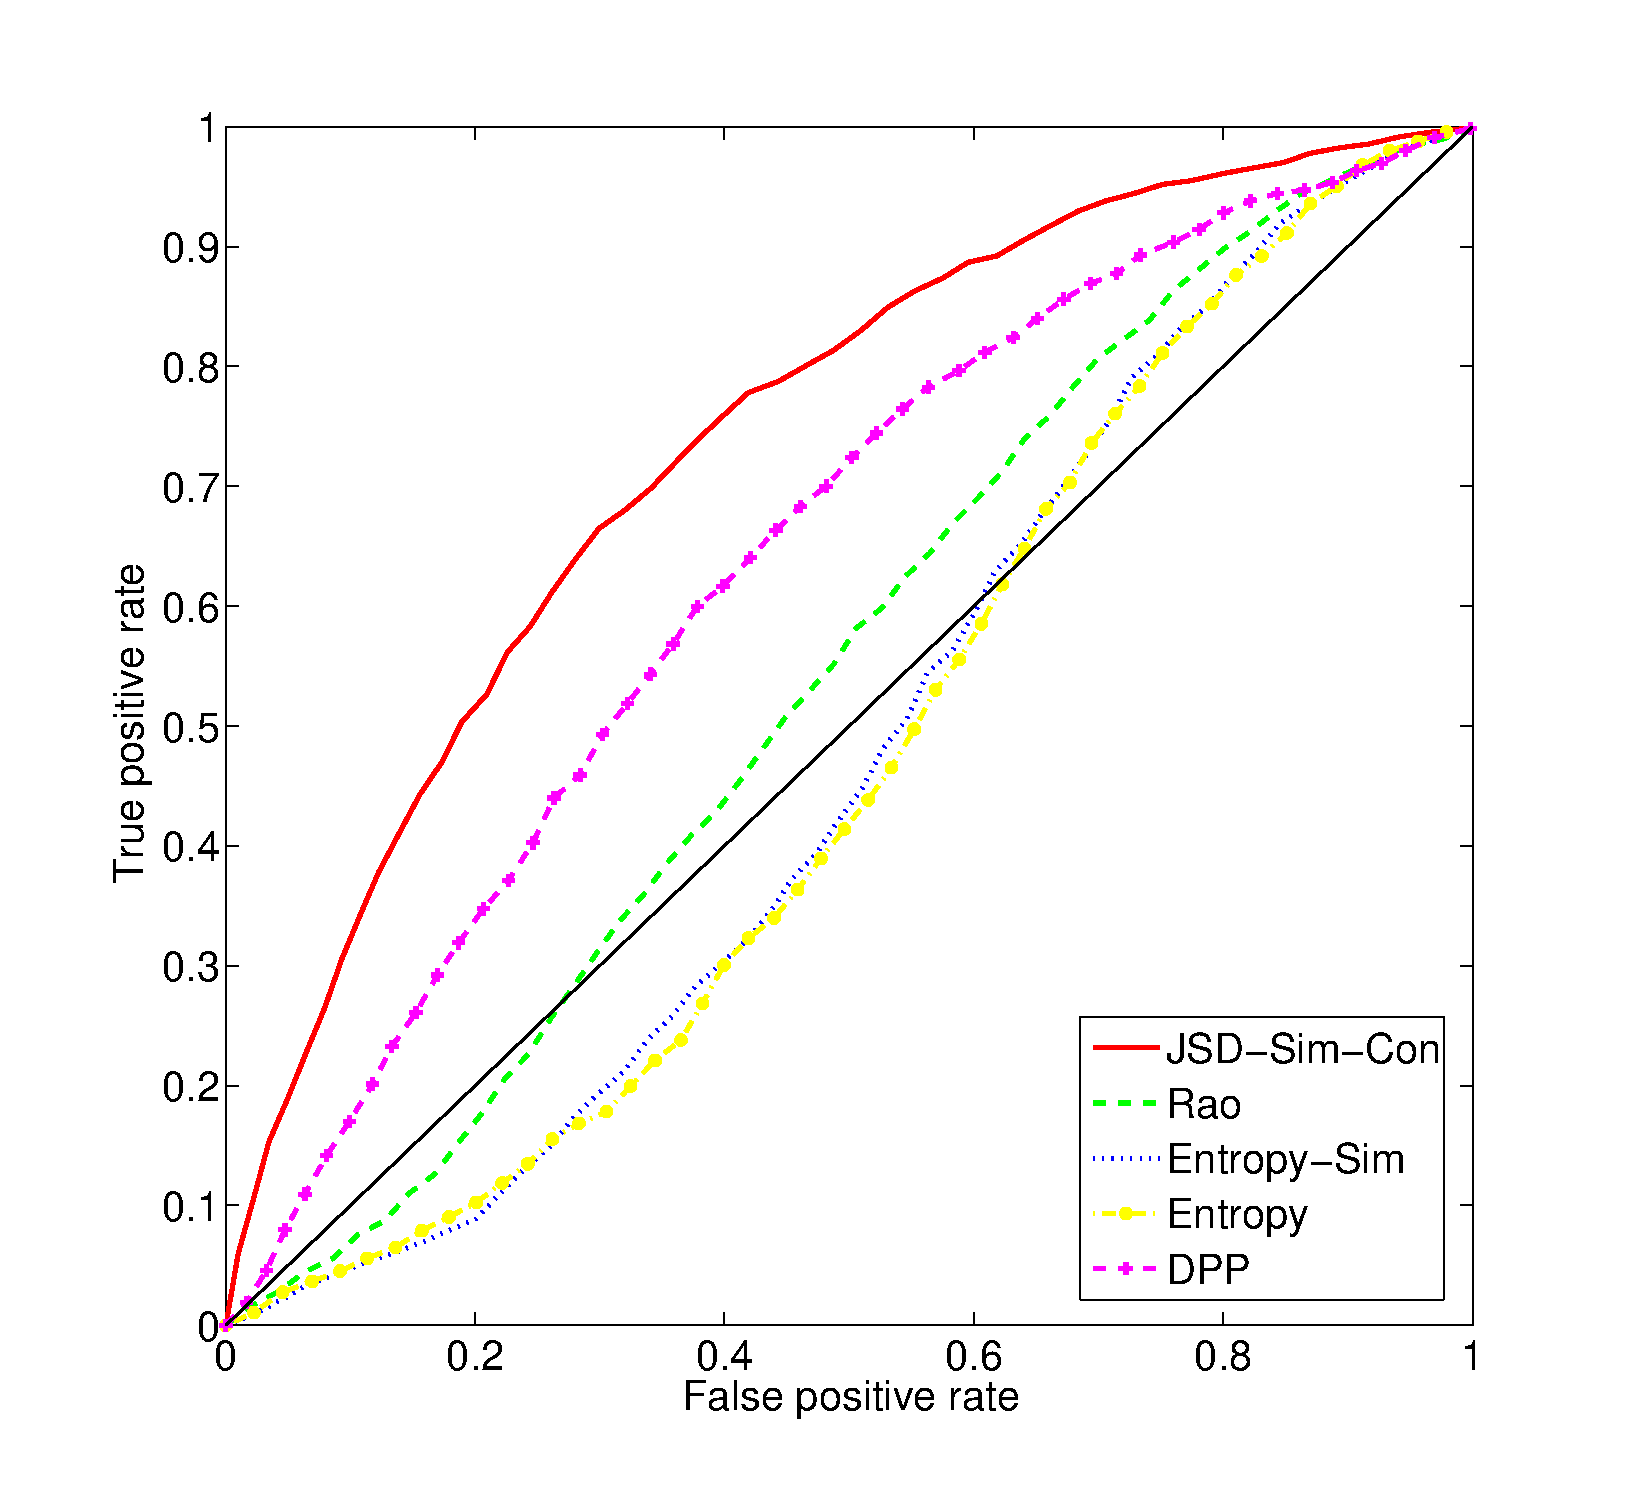
\includegraphics[width=0.45\textwidth]{figures/phonecases-comparison-new.eps}
    % \caption{}
\hspace{4mm}
  \end{subfigure}%
  ~
  \begin{subfigure}
(b) \hspace{-1mm}
    \centering
    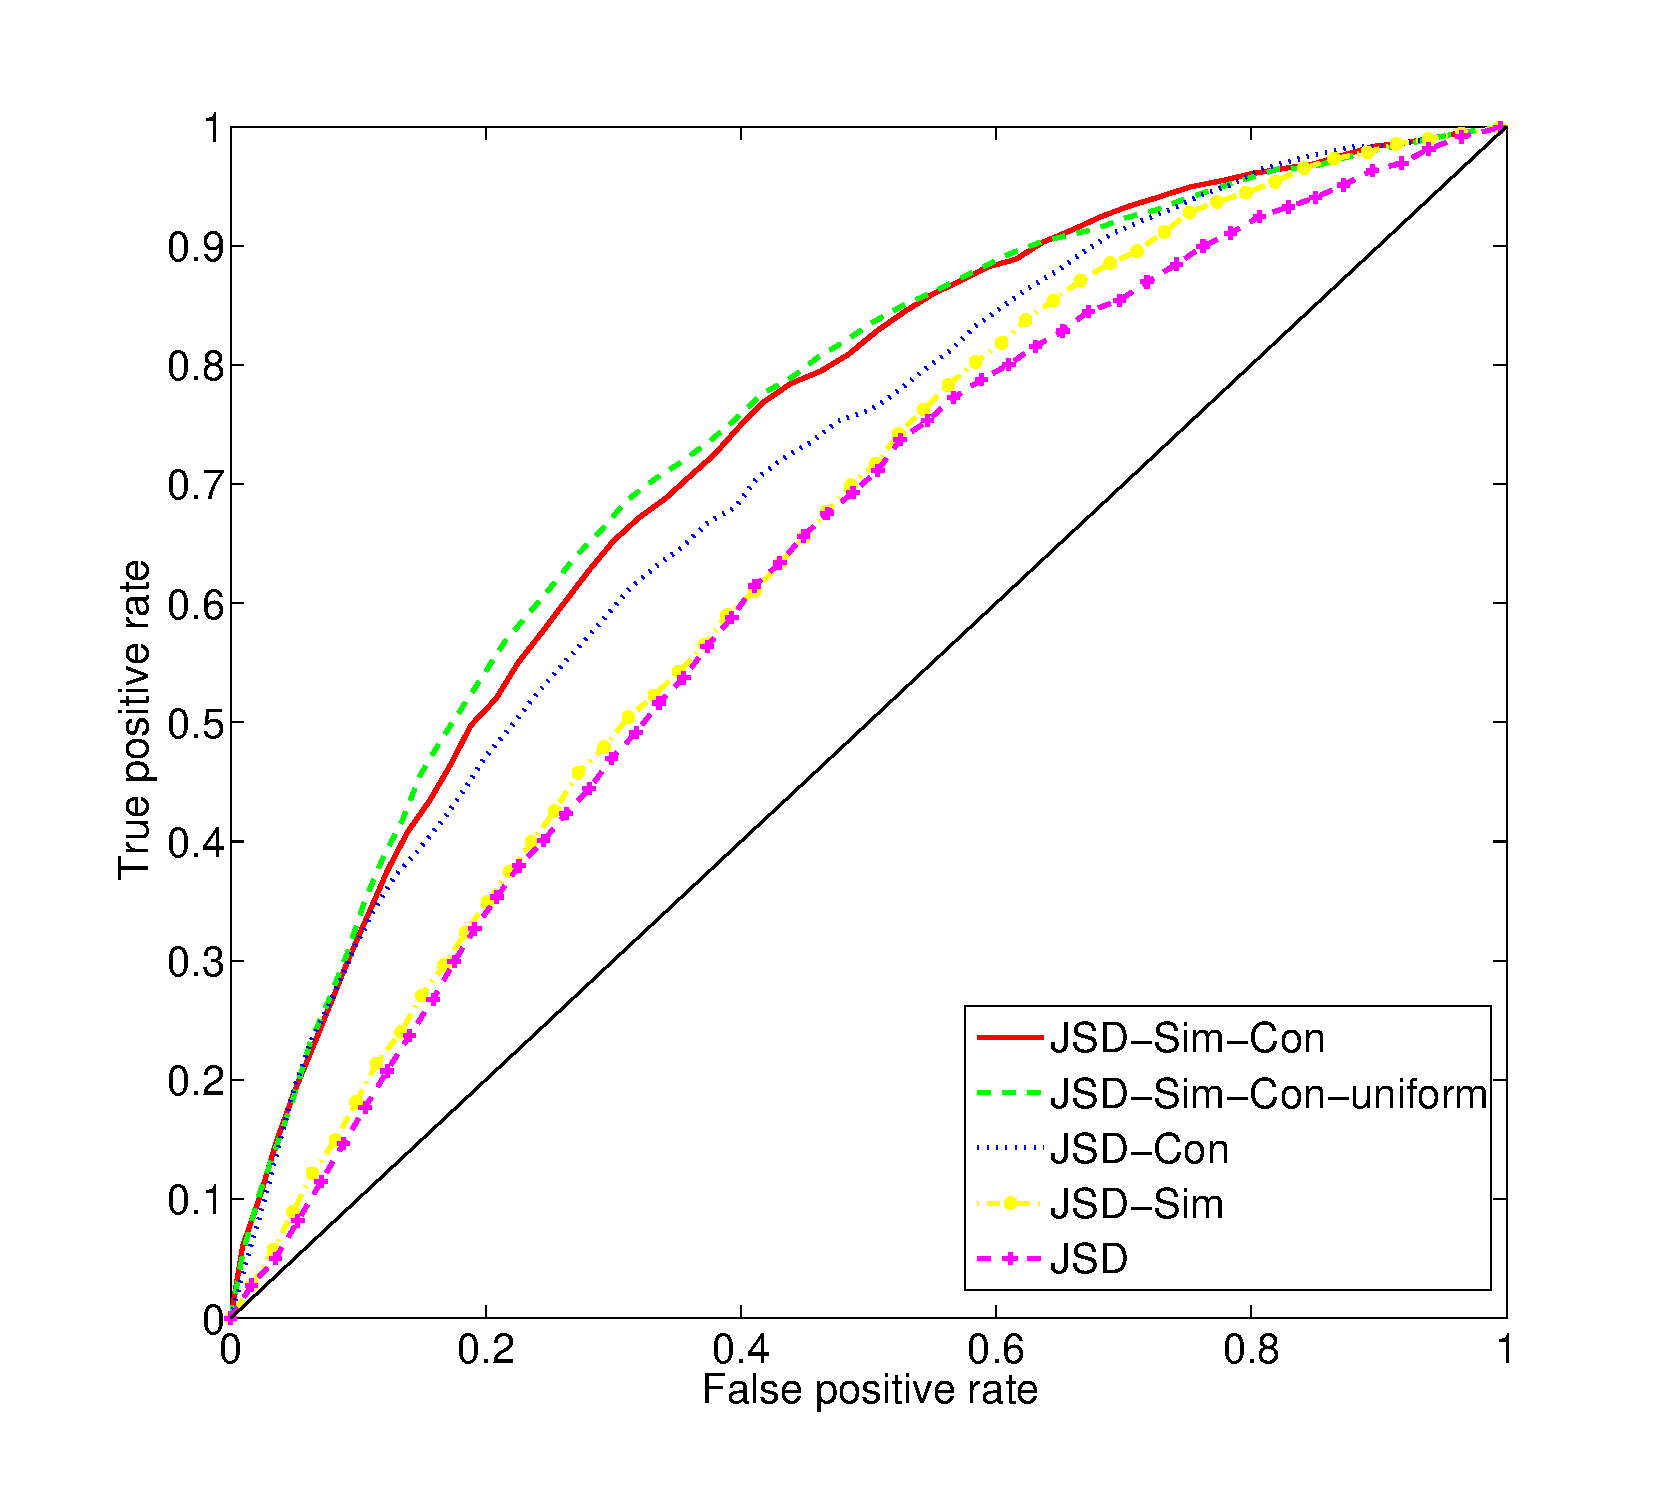
\includegraphics[width=0.45\textwidth]{figures/phonecases-breakdown-new.eps}
%    \caption{}
  \end{subfigure}
  
  \begin{subfigure}
(c) \hspace{-1mm}
    \centering
    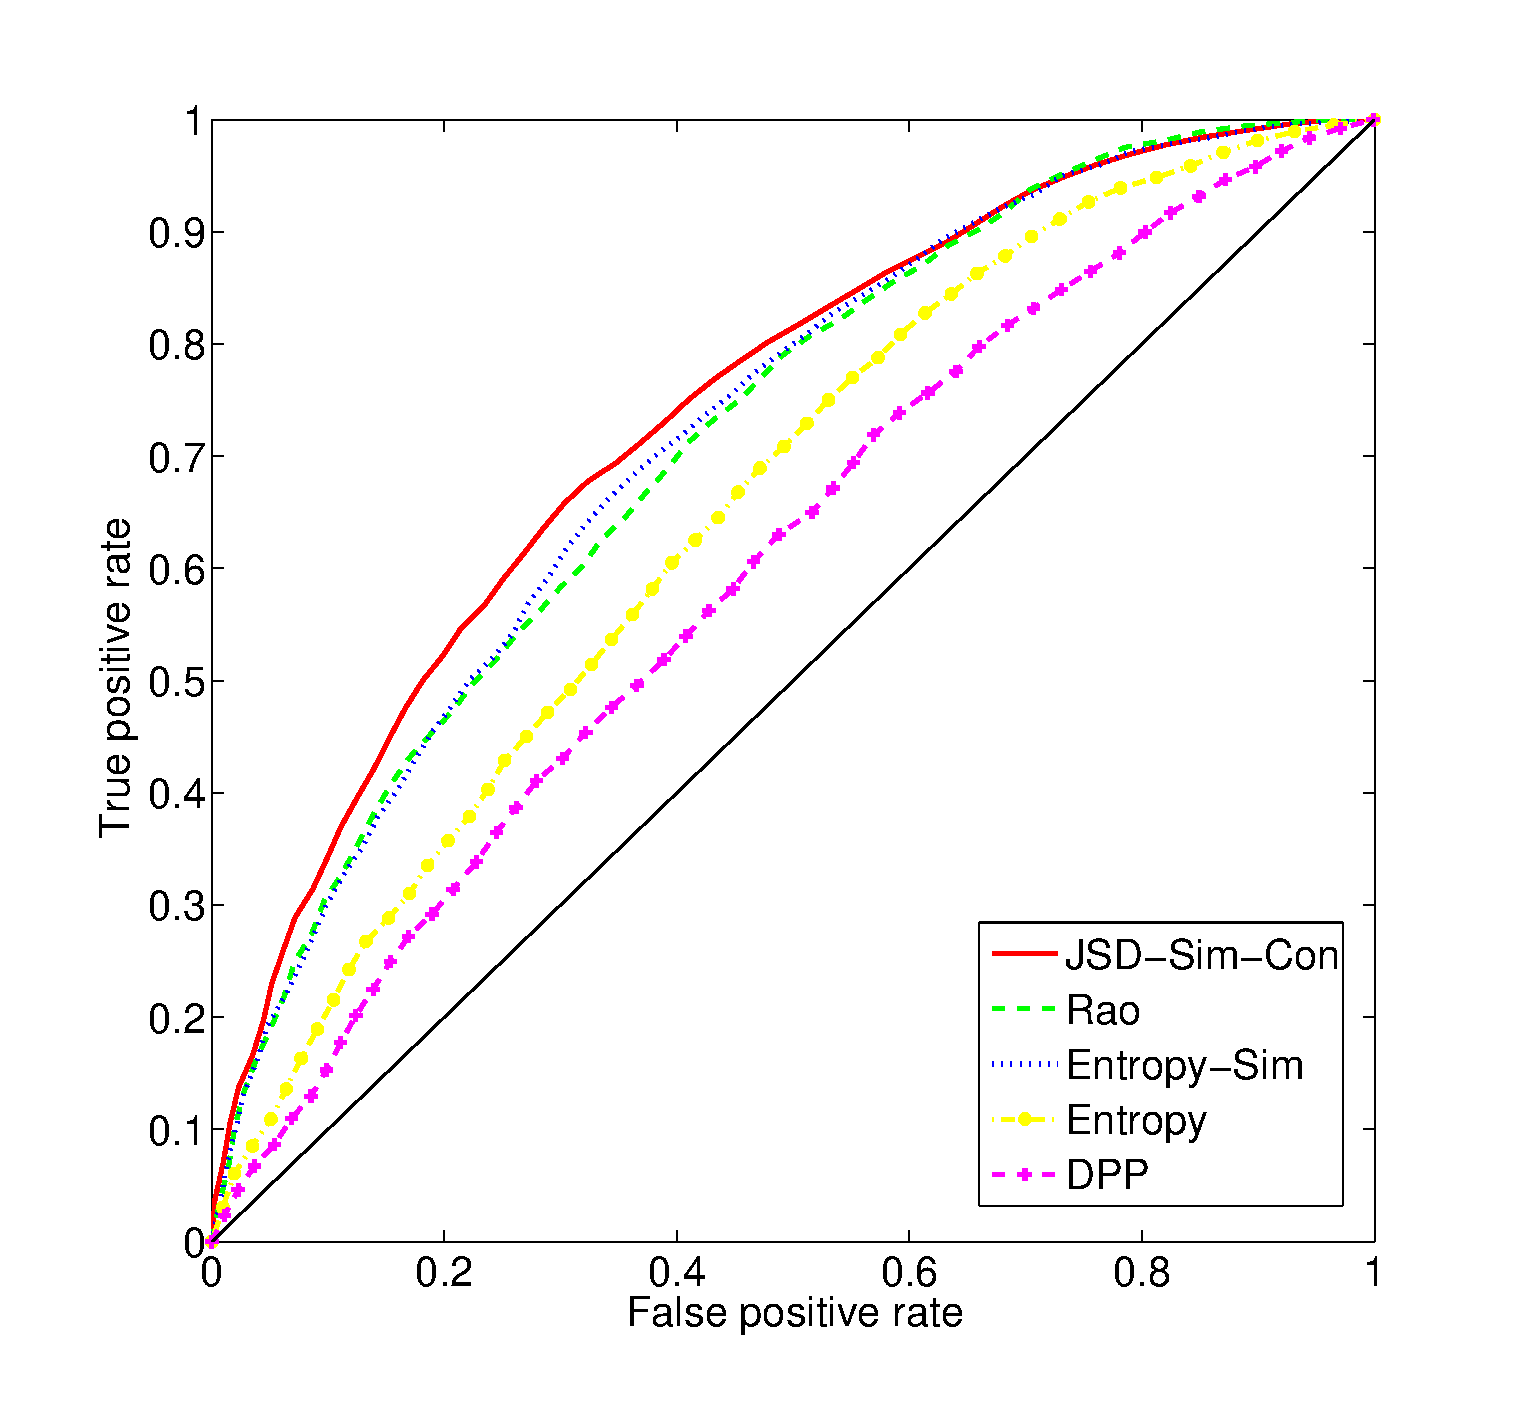
\includegraphics[width=0.45\textwidth]{figures/nsf-comparison-new.eps}
 %   \caption{}
\hspace{4mm}
  \end{subfigure}%
  ~
  \begin{subfigure}
(d) \hspace{-1mm}
    \centering
    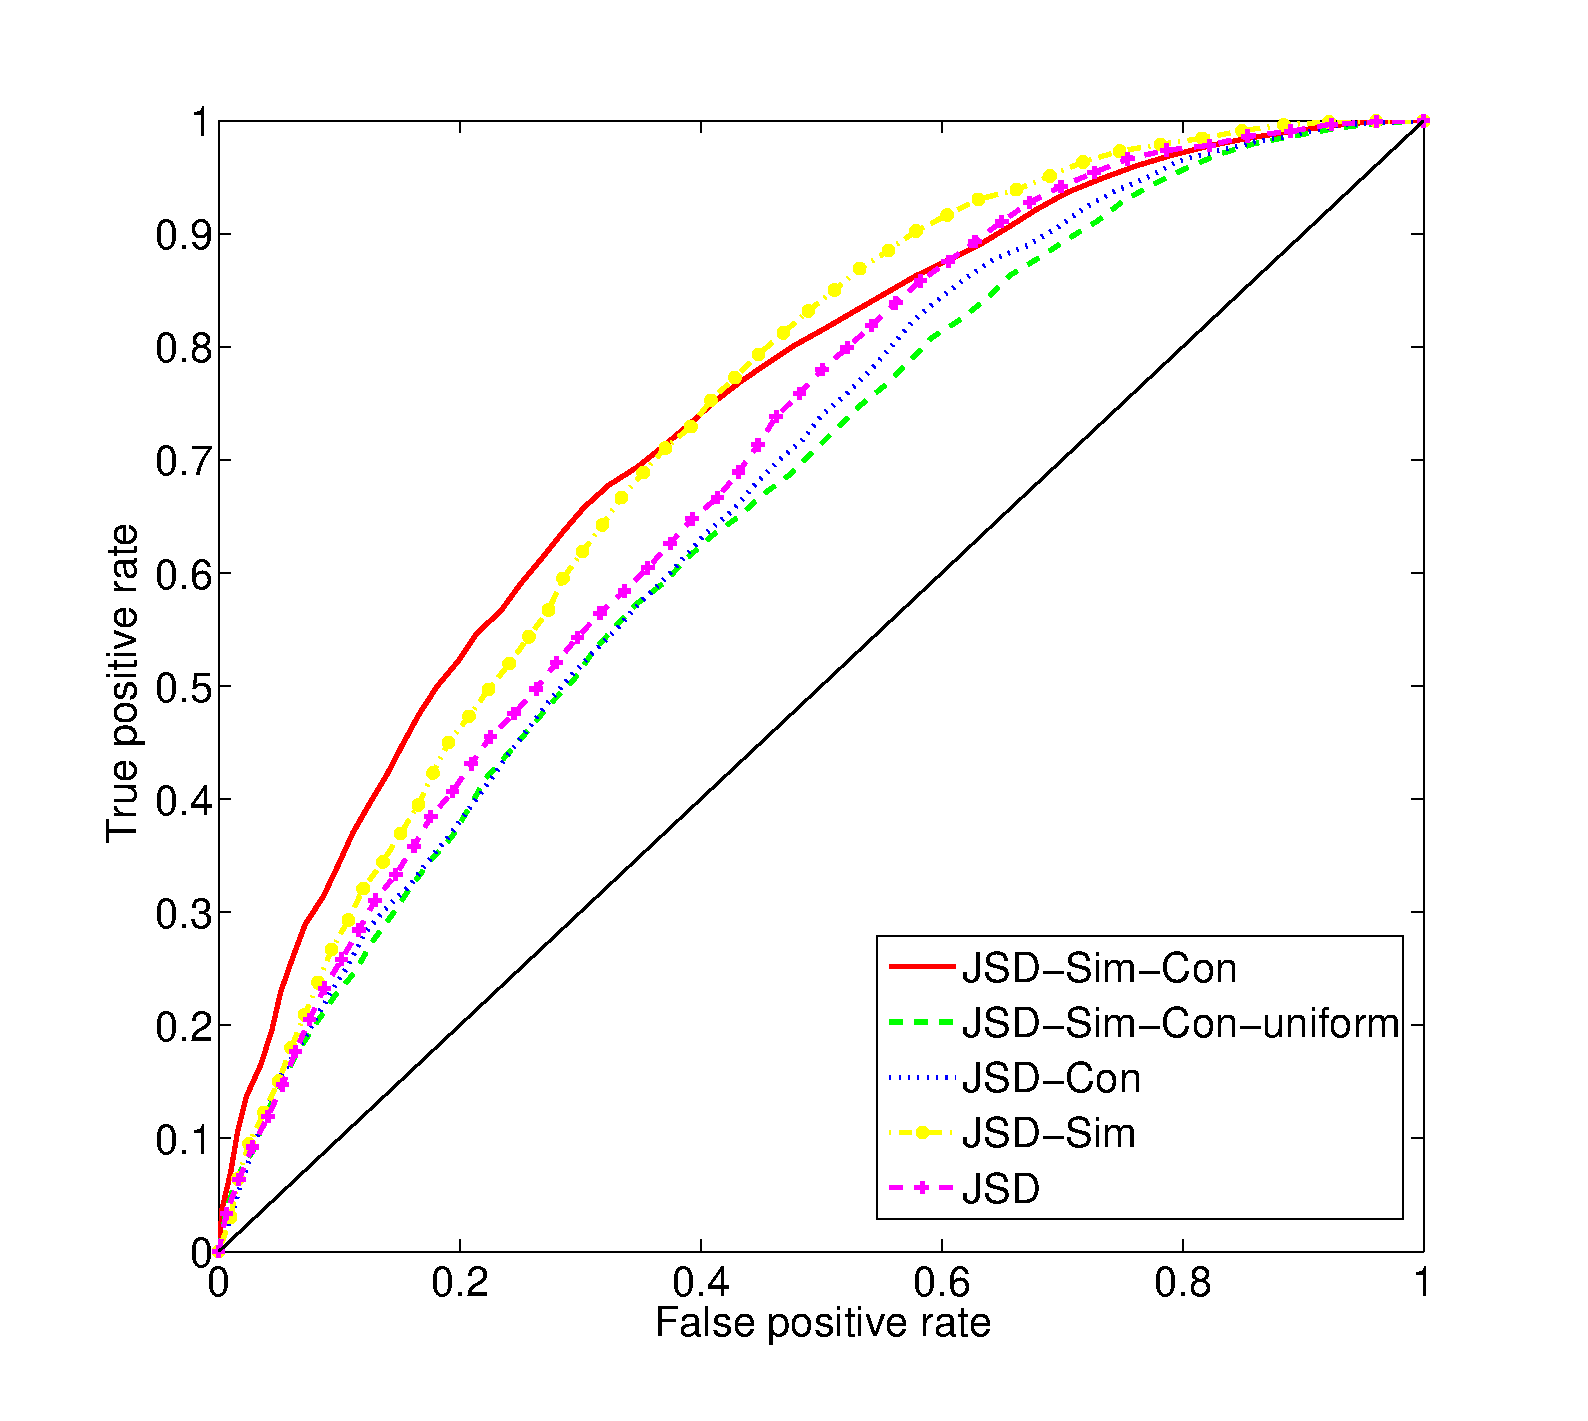
\includegraphics[width=0.45\textwidth]{figures/nsf-breakdown-new.eps}
 %   \caption{}
  \end{subfigure}

  \caption{ROC curves presenting the results of experiments on
 the eBay dataset (a,b) and NSF proposal dataset (c,d). The
 comparison plots (a,c) show the results for our approach (JSD-Sim-Con)
 against other methods, while the plots (b,d)
 show different variations of our approach. }
\label{fig:roc-curves}
\end{figure*}

%   \begin{table*}[t]
% \begin{center}
% \begin{tabular}{CC}
% 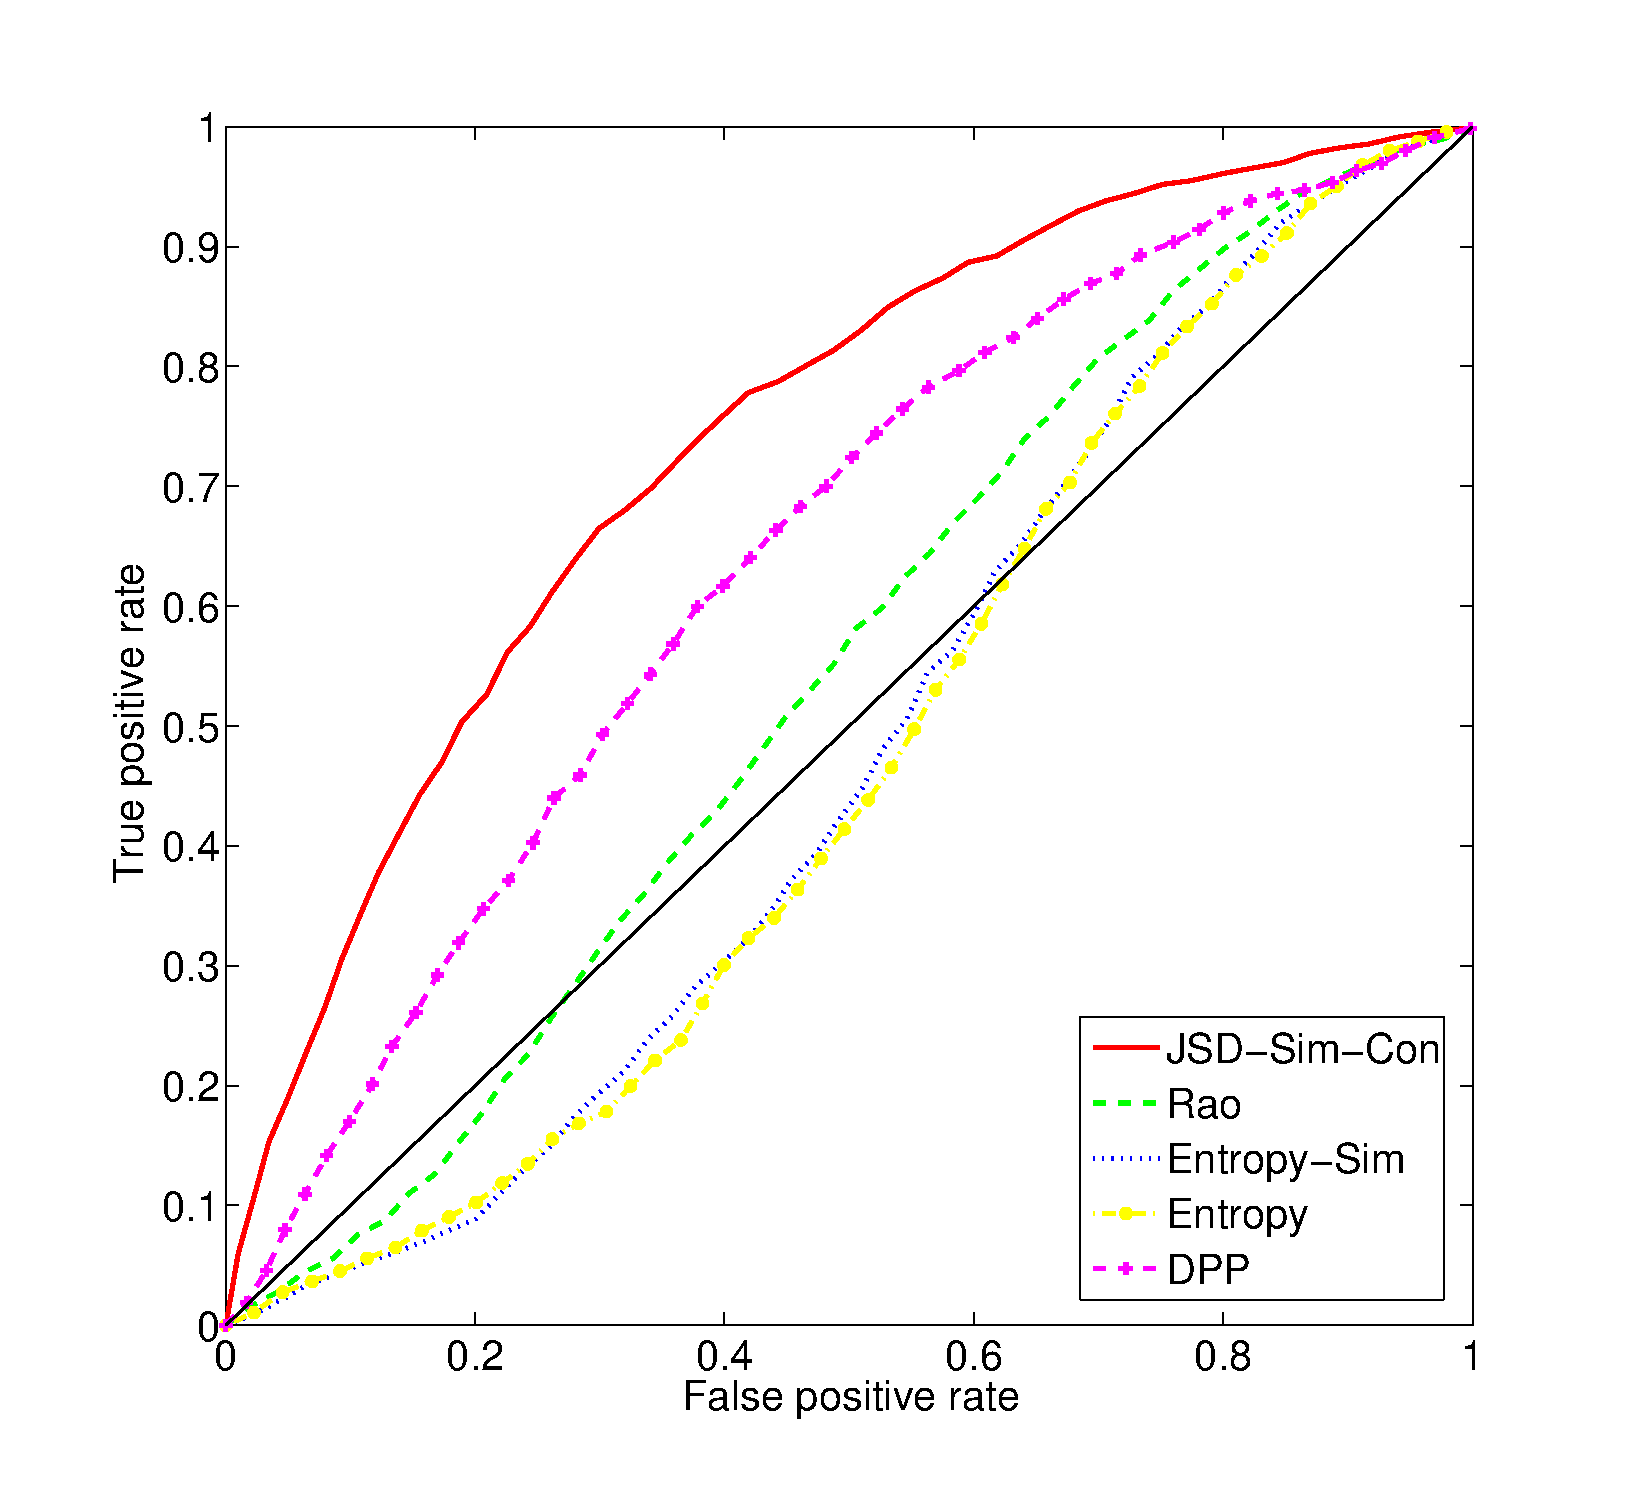
\includegraphics[height=6.5cm]{figures/phonecases-comparison-new.eps}&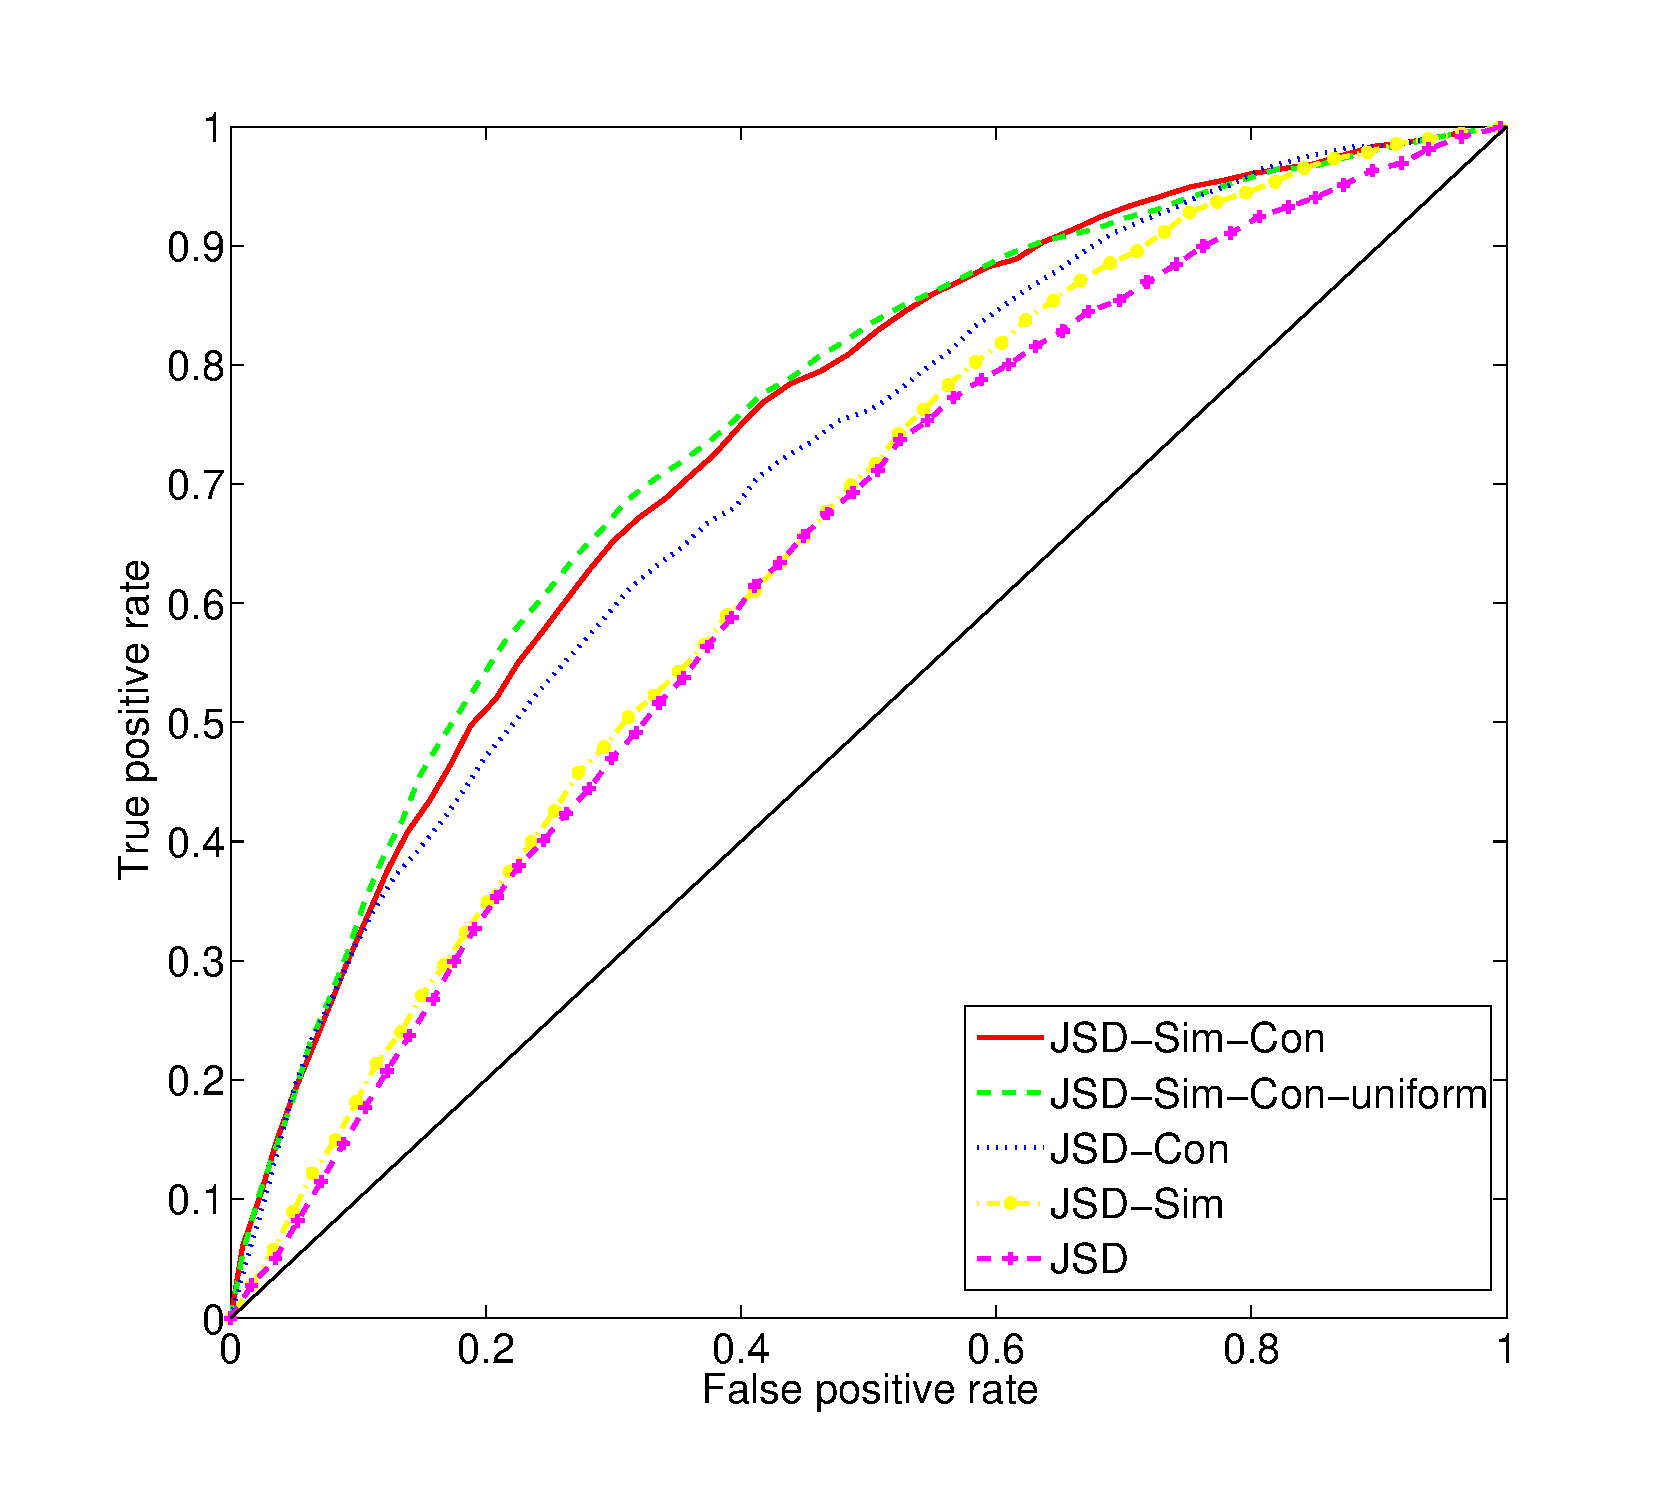
\includegraphics[height=6.5cm]{figures/phonecases-breakdown-new.eps}\\
% (a) & (b)\\
% 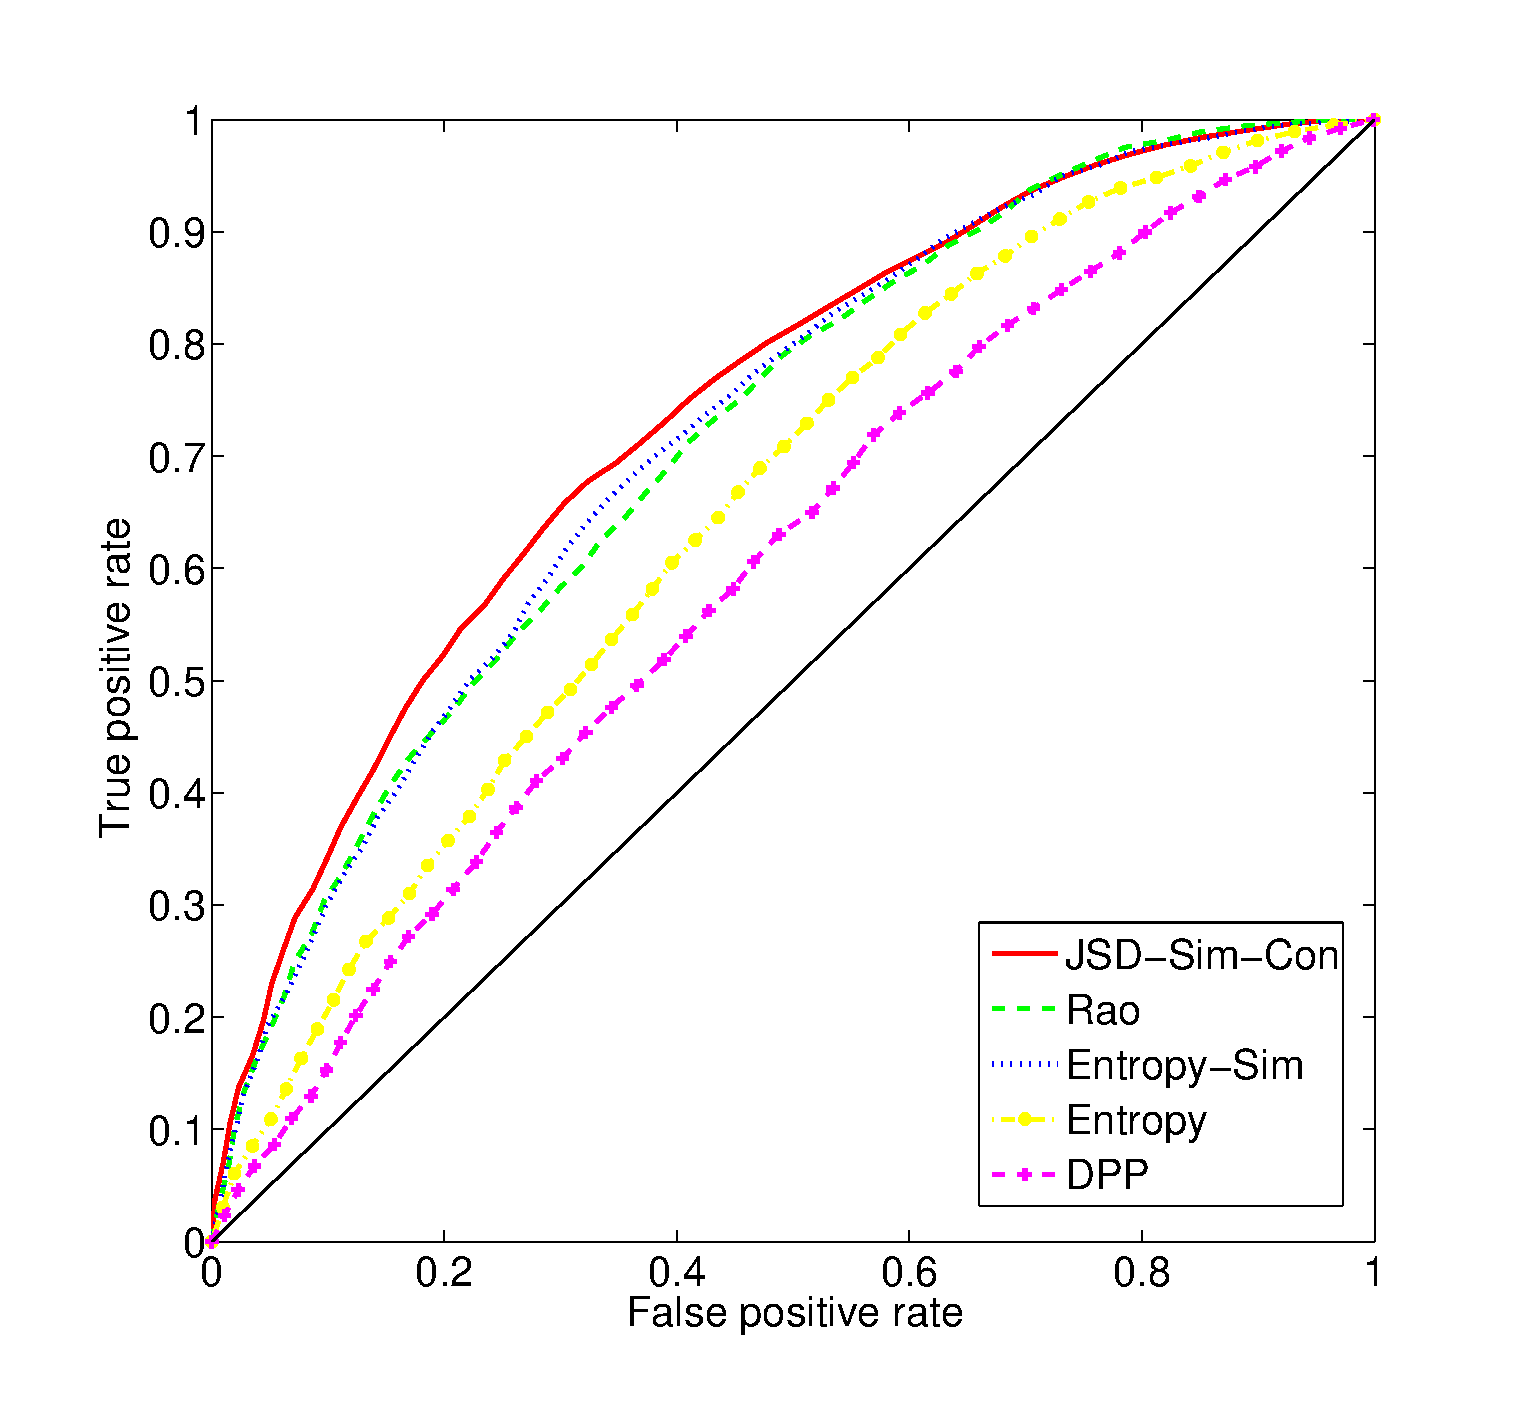
\includegraphics[height=6.5cm]{figures/nsf-comparison-new.eps}&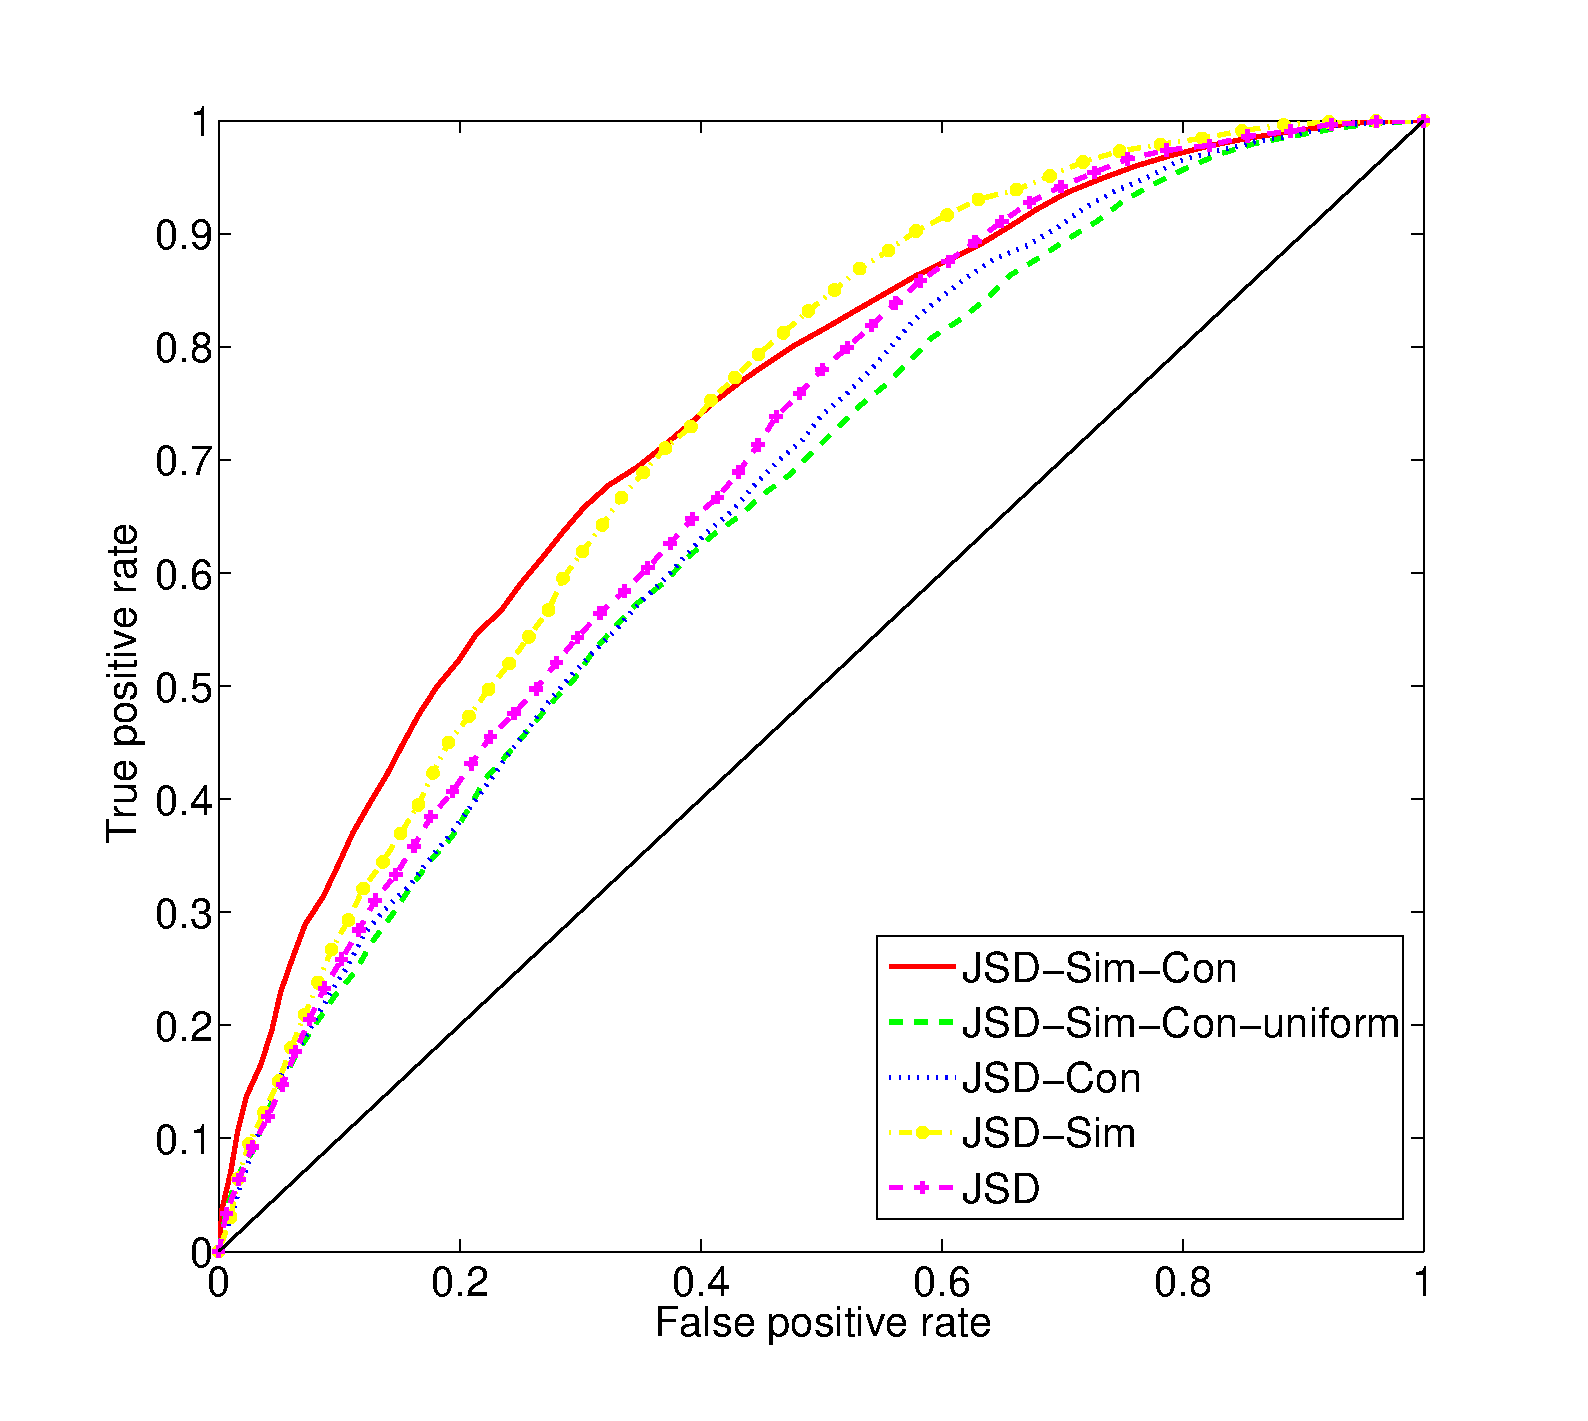
\includegraphics[height=6.5cm]{figures/nsf-breakdown-new.eps}\\
% (c) & (d)\\
% \end{tabular}
% \end{center}
% \caption{ROC curves presenting the results of experiments on
% the eBay dataset (a,b) and NSF proposal dataset (c,d). The
% comparison plots (a,c) show the results for our approach (JSD-Sim-Con)
% against other methods, while the plots (b,d)
% show different variations of our approach. }
% \label{fig:roc-curves}
% \end{table*}



%%%%%%%%%%%%%%%%%%%%%%%%%%%%%%%%%%%%%%%%%%%%%%%%%%%%%%%%%%%%%
%%%%%%%%%%%%%%%%%%%%%%%%%%%%%%%%%%%%%%%%%%%%%%%%%%%%%%%%%%%%%
%%%%%%%%%%%%%%%%%%%%%%%%%%%%%%%%%%%%%%%%%%%%%%%%%%%%%%%%%%%%%

\section{Experiments}
\label{sec:experiments}


Through the use of experimental results, we aim to prove several
claims made in this paper. First, we show that in some domains of
e-commerce measuring text diversity for product titles is a valid
approach for discovering interestingness. To that end, we present the
unsupervised evaluation of diversity scores against human-made
interestingness labels for products in an eBay dataset of iPhone
cases. Second, we evaluate our proposed text diversity measure against
several baselines on the dataset based on NSF grant proposal
abstracts, to show that our model does in fact measure
diversity. Finally, as part of our model, we proposed a method for
extracting topic-distributional representations of words and
sentences. Even though it is not the main goal of the paper, we were
interested to see how these representations perform as feature vectors
in a supervised setting. To that end, we used the eBay product
dataset again, comparing against other text embedding techniques.

\subsection{Datasets}
\label{sec:datasets}

We used the following two datasets in our experiments: 

{\bf Interesting iPhone cases}.
In this dataset, we collected a number of interesting (positive) and uninteresting (negative) iPhone case product titles as follows. For generating positive examples, one natural choice was exploiting the data hosted by Pinterest. By definition, it is fair to assume that anyone who pins a product on Pinterest has found it interesting to some degree. The more a pin is engaged by the users, the more interesting is the product to those users. Although Pinterest data is biased by the demographic of its users, it is a publicly available dataset and is a more natural choice compared to collecting interesting products using crowd sourcing such as  {\em Amazon Mechanical Turk (AMT)} where it would be more subject to demographic biases. We built a pipeline for generating interesting eBay products illustrated in Figure~\ref{fig:pinterest-pipeline}.  In the first stage, we periodically crawl pins from Pinterest. In the next stage we filter the pins which do not have rich textual content and then rank the remaining pins using a score computed from the number of {\em repins}, {\em likes}, and {\em comments}. In the next stage, we trained a linear-chain {\em Conditional Random Field (CRF)}~\cite{Lafferty:2001:CRF:645530.655813} for extracting product related keywords from a set of highly ranked pins produced in the previous step. The final set of product related keywords  is then used to find a match in the eBay inventory. 

For generating the uninteresting iPhone case dataset (negative examples), we
hired workers from {\em AMT} to label a collection
of nearly 20,000 iPhone cases on {\em eBay}.  We then pulled our final dataset from the annotated by selecting only those instances where the annotators all labeled it as uninteresting. 

The final dataset consists of $2179$ positive and $9770$ negative instances
for a total of $11,949$ instances. For each instance, the product title of
the corresponding {\em eBay} listing was used as the input. In this case we are
dealing with very short text snippets, usually 10 to 12 words each. To
train a topic model, we used a larger, more broader set of about
$2$ million product titles, grouped based on {\em eBay} categorical information into about $8,000$
documents of approximately $200$ titles each. We used the Mallet LDA
implementation to learn a topic model with $400$ topics.


%{
% We used insights from 
% interesting iPhone cases found on {\em Pinterest} and {\em eBay's}
% user behavior data in order to generate a balanced data-set.  
% We then pulled our final dataset from the annotated by selecting only
% those instances where the annotators all labeled it as 
% positive (i.e., interesting) or negative (i.e., uninteresting). The
% final data-set consists of 2179 positive and 9770 negative instances
% for a total of 11,949 instances. For each instance, the product title of
% the corresponding {\em eBay} listing was used as the input. In this case we are
% dealing with very short text snippets, usually 10 to 12 words each. To
% train a topic model, we used a larger, more broader set of about
% 2 million product titles, grouped based on {\em eBay} categorical information into about 8,000
% documents of approximately 200 titles each.
%}

{\bf {\em NSF} abstracts}. For the second dataset we used a set of
61,902 National Science Foundation 
Scholarship proposal abstracts (see~\cite{bache:2013} for more
details) to evaluate how our diversity measure 
compares to other methods on larger pieces of text. We used this set
for training a topic model, however to get labeled data, we had to
generate artificial examples, by randomly mixing pairs of abstracts that we
could expect to be either similar (small diversity) or very different
(high diversity), based on the available meta-data, and labeling them accordingly. We generated 5,000 of
those examples with positive and negative labels evenly
represented. For this experiment, we trained a separate topic model with $300$ topics
based on the original NSF abstracts. To give better intuitions for
this setting, Table \ref{tab:nsf-examples} presents two example
abstracts - one, which the model deemed diverse, with score 1.25, and
a much less diverse one, with score 0.71. Note, that theoretically the
diversity may be anywhere between $0$ and $\log(|T|)\approx 5.7$, but
in practice, almost all of the documents fell into the range of $0.6$
to $1.3$. The table shows top three topics that the model associated
with each of the two example abstracts. For the more diverse abstract, the
topics (Linguistics, Design and Decision-Making) are relatively dissimilar,
while for the less diverse one (Algebraic Geometry, Combinatorics and
Foundations) they are closely related to each other, hence the lower score.  

\begin{table*}[t]
\renewcommand{\arraystretch}{1.3}
\caption{Examples of NSF Abstracts:
(left) example of an NSF proposal found by our approach to be more diverse (inter-disciplinary proposal); (right) example of an NSF proposal mostly centered on a single area.}
\label{tab:nsf-examples}
\centering
\begin{tabular}{r|l|r|l}
\multicolumn{2}{c}{\bfseries High
  Diversity}&\multicolumn{2}{c}{\bfseries Low Diversity}\\
\hline\hline
\multicolumn{2}{c|}{{\bf Title}\hfill\quad {\em Linguistics-Based Preference Information Modeling for Design
Decision-Making}} & \multicolumn{2}{c}{{\bf Title}\hfill\quad {\em Ramsey Theory: Central sets and related
combinatorially rich sets}}\\
\hline
Main Topics & Top 5 words for topic, from LDA & Main Topics & Top 5 words for topic, from LDA\\
\hline
Linguistics & language, linguistic, english, speakers, words &
Algebraic Geometry& theory, algebraic, geometry, representation,
algebra\\
Design & design, engineering, principles, implementation,
methodology & Combinatorics & theory, graph, problems, discrete, combinatorial\\
Decision-Making &decision, making, uncertainty, risk, choice &
Foundations& theory, understanding, fundamental, framework, general
\end{tabular}
\end{table*}

% Three main topics: Language (138), Design (37), Decision-Making (208).

% Language (138): 1912        5659       11148       20337        4655        4784        5091        1044         334        6809
% language languages linguistic english speakers words word
% linguistics documentation translation
% Design (37):        212         162        5031        2667       1790        2781        1791         290         192        1489
% design engineering designs designing principles implementation
% methodology objective tools designers
% Proposal ? (253):         1105         291        5970        5414        5070        5674        3609       15718        2137        2508
% public award recovery act funded american law reinvestment employ
% funds 
% Decision-Making (208)        1063         875         898         874         449         788        3317        3569          32         792
% decision making decisions uncertainty risk make choice choices
% research individual

% Algebraic Geometry (41)          8         612          78         611         636      827         820        1347         829          12
% theory algebraic geometry representation algebra algebras quantum
% geometric mathematics study
% Combinatorics (28)           8        1683           7        1660         510        1338        1663          44          45         734
% theory graph problems graphs discrete combinatorial complexity
% applications areas set
% Theory (223)          8         914        2118          77         330         740         151        4049        1983         200
% theory theoretical theories understanding fundamental framework
% general string foundations ideas


% 0900255	07/01/2009	Division of Civil, Mechanical, and Manufacturing Innovation	ENGINEERING DESIGN AND INNOVAT; 	Linguistics-Based Preference Information Modeling for Design Decision-Making	This award is funded under the American Recovery and Reinvestment Act of 2009 (Public Law 111-5). The objective of this research award is to model the preference information embedded in natural language engineering design texts in order to identify linguistic forms of preference that will form the basis for a decision-making model that supports comparison of computed decisions to actual decisions. One view of the product design process is that it is driven by designers who have preferences for alternatives within a set of possible design choices. Such preference information is implicit within engineering design texts, but can be difficult to extract from unstructured information. The challenge is in linguistically modeling these preferences and mapping them into a mathematical model suitable for supporting design decision-making. Work will identify linguistic forms of preference, produce a comprehensive 'preference lexicon', develop formal mathematical models of preferences, and generate a decision-making model so that computed decisions can be compared with actual decisions to verify their validity.  If successful, this work will have impact across many industries, including product development, automotive, aerospace, and the military, due to the fundamental role of decision-making in the engineering design process. This research is intended to advance fundamental understanding of the language of design, in particular how preferences are expressed. In turn, this will further basic knowledge of the subjective aspects of decision-making and move towards the development of usable, effective decision support methods. The result will be an approach for imputing preference information as well as decision information from unstructured design texts that draws on both design language models and probabilistic extraction. Graduate students will learn about this work through an interdisciplinary, project-based class on decision-making in engineering design. A diverse group of undergraduates will have hands-on research experience with this work the Undergraduate Research Opportunities Program.


% 1160566	07/01/2012	Division of Mathematical Sciences	PROBABILITY; Combinatorics; 	Ramsey Theory: Central sets and related combinatorially rich sets	Ramsey Theory is that part of combinatorics that deals with the question of what sort of homogeneous structures one can expect to find in some one cell of a finite partition of a specified set (or sometimes in any suitably "large" subset). For example, the simplest nontrivial instance of the infinite version of Ramsey's Theorem says that whenever the two-element subsets of the set N of positive integers are finitely colored, there must be some infinite subset of N all of whose two element subsets are the same color. Many years ago, the principal investigator proved that whenever N is finitely colored, there must exist in one color an infinite sequence together with all of its finite sums of distinct terms without repetition. The original proof was elementary, but very complicated. Subsequently, other proofs were found that were less complicated. But in 1975, F. Galvin and S. Glazer showed that this "Finite Sums Theorem" is a completely trivial consequence of the fact that the Stone-Cech compactification of N can be given an algebraic structure extending ordinary addition which makes it a compact right topological semigroup, and therefore has idempotents. Sets with the property that they contain all the finite sums from a sequence are called IP sets. By virtue of the connection discovered above, a set is an IP set if and only if it has an idempotent in its closure in the Stone-Cech compactification of N. Those that have special idempotents which are called "minimal" in their closure are "central" sets. These sets have much stronger properties, many of which are consequences of the Central Sets Theorem. But central sets have a very complicated elementary description. Sets which satisfy the conclusion of the Central Sets Theorem are called "C-sets", and are much easier to describe in an elementary fashion. The proposed investigation of these various algebraically characterized large subsets of N should continue to yield new Ramsey-theoretic results.  A significant portion of the funds in this grant will provide support for graduate students at Howard University, an historically black university. In particular, the grant will provide stipends for three Ph.D. students, two of whom are black Americans, both female. This project will therefore be instrumental in training mathematicians who come from a population that is severely underrepresented within the population of US mathematicians.


\subsection{Unsupervised Setting}
\label{sec:unsupervised-learning}

We evaluated our text diversity model in an unsupervised learning task
on both datasets.
We implemented our model as described in
Sections~\ref{sec:information-diversity}-\ref{sec:topic-similarities} (labeled by {\em
    JSD-Sim-Con}) and compared it against a few 
baselines: Shannon entropy, Rao Diversity and a measure
based on Determinantal Point Processes.
The Shannon entropy has
been previously tested as a measure of document diversity with quite
underwhelming results in \cite{bache:2013}, where the authors proposed 
Rao diversity as a better solution, which incorporates the topic similarity
information to provide better accuracy. We suspected that
poor performance of entropy might be due to a suboptimal choice of
topic distribution, which led to our topic similarity
method. This technique can be used on any topic distribution
by simply multiplying it by the topic similarity matrix $\cS$. We present the performance of entropy with - and 
without - the topic
similarity transformation to verify that this approach improves the results not
only for Jensen-Shannon Divergence, but for other measures as well.
Both for the entropy and Rao diversity, we generated topic
distributions by inferring them for each instance, based on the LDA
model, using the standard functionality from Mallet.

Determinantal Point Processes (DPP) have recently gained popularity as a
useful tool for sampling diverse subsets, with many applications
(see~\cite{kulesza:2012} for more details). We were interested to see
if they can also be useful for 
measuring the diversity of a set provided as input. Given a set of
instances described as feature vectors $U=\{v_i\}_{i=1}^N\subset \rr^T$, DPP defines a
sampling model for selecting a subset of $S=\{v_{i_j}\}_{j=1}^k$, by
setting the probability of $S$ proportional to the determinant of the
Gram matrix corresponding to those vectors. One might therefore
consider this determinant to be a good measure of set diversity,
because, intuitively, a more diverse set should have a higher
probability. The problem with this, however, is that determinants are
computationally unstable and very sensitive to local changes. For
example, if any two instances happen to have identical vector
representations, that immediately forces the determinant to $0$, even
though a set may be otherwise very diverse. We decided to use
another measure derived from a DPP. Instead of looking at a set $S$
(in our case, a set of words) as a sample from a larger set, we can
imagine sampling from $S$ itself. In that case, the average size of
the samples tells us how many significantly different words there are
in the given text. Fortunately, the expected sample size can be
computed from the eigenvalues of the aforementioned Gram matrix, as
discussed in \cite{kulesza:2012}. Two aspects of the feature
vectors are relevant for the DPP. The length of the vector represents
the relevance of the corresponding word, while the direction is
responsible for determining the pairwise similarities. For the
direction, we used the distributional representations from 
our model. For the vector lengths, we tried two versions: all
unit lengths (i.e. no preference), and using the importance values from
Definition \ref{mixture}. One drawback of the expected
DPP sample size is that it is correlated with the length of a
document. However, within each of our datasets, the instances have roughly
similar length.

Figures \ref{fig:roc-curves} (a) and (c)
present ROC curves comparing all of the diversity measures for each dataset.
In either case it can be observed
that our approach outperforms the other baselines, with an AUC
around $0.73$. Moreover, for the {\em eBay} dataset the other measures
give poor results. This can be explained as follows: since the
text snippets are short, the LDA may yield a poor topic inference for
such short text and as a result all measures using topic inference
would perform poorly. Our technique only relies on the topic model for
computing the distributional representations of words, so LDA can be
trained on a separate dataset and does not have to be affected by the
length of documents in the test set.
 The DPP-based measure does have some correlation
with the labels for both datasets, although not particularly
high. Interestingly, for the eBay dataset, unit vector lengths
performed better, while for NSF, importances gave an improvemet (in
each case, only the better result was
plotted). Another interesting observation is that 
Shannon entropy on the NSF dataset performs much better when applied
to distributions transformed using topic similarity information. In
fact, in our experiments it did better than Rao diversity, which also
used the same topic similarity matrix. This shows that the
transformation proposed in Section~\ref{sec:topic-similarities} is an
effective way of incorporating topic similarity information when
measuring diversity.
\begin{figure}
\begin{center}
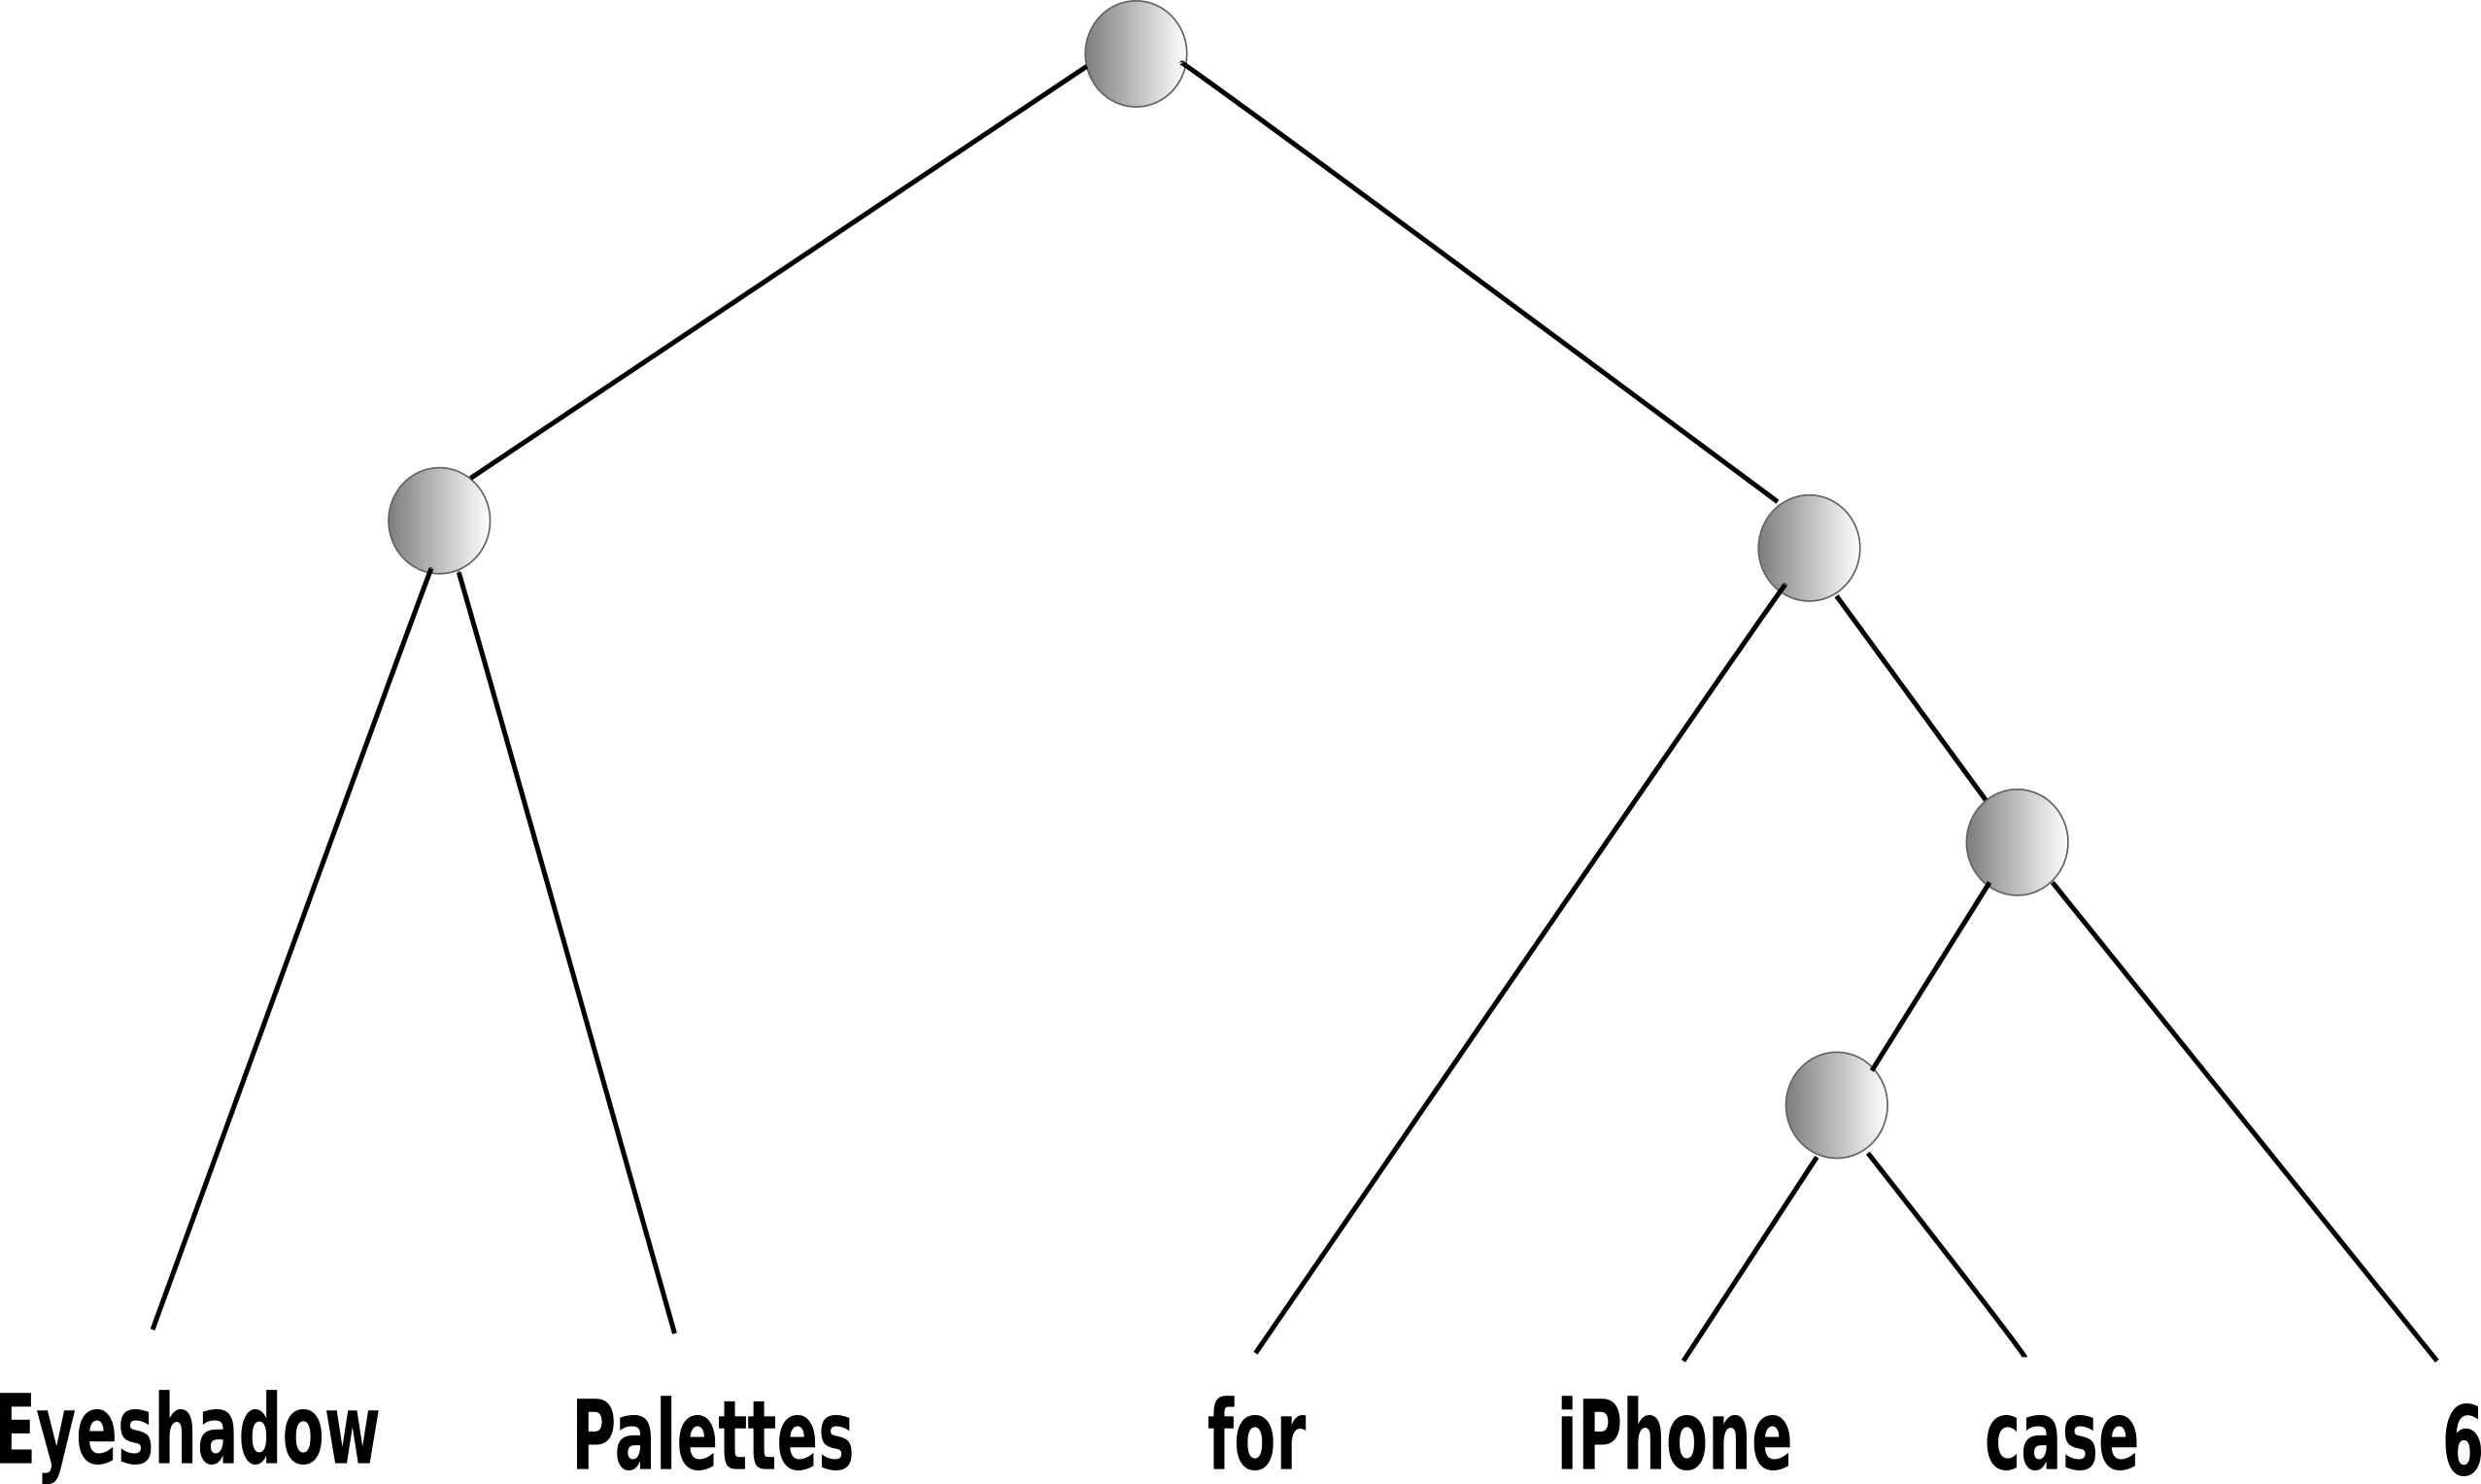
\includegraphics[width=8.5cm]{figures/RAE-example.png}
\caption{RAE tree learned for the product: {it Black Qi Standard Wireless Charging Charger Receiver Case For iPhone 5 5G}. Note how RAE learns to merge different concepts separately and merges them until very last step into the root node.}
\end{center}
\label{fig:rae-example}
\end{figure}

\begin{table*}[t]
\renewcommand{\arraystretch}{1.3}
\caption{Classification results for the eBay dataset.}
\label{tab:classification-results}
\centering
\begin{tabular}{l||c|c|c|c}
&Precision & Recall & F1 & Accuracy
\\ \hline \hline
JSD Features         &$\mathbf{0.714}\pm 0.015$&$0.597\pm 0.016$&$0.650\pm
0.014$& $\mathbf{0.8828}\pm 0.0045$\\
RAE Features         &$0.676\pm 0.005$&$\mathbf{0.666}\pm 0.030$&$\mathbf{0.671}\pm
0.013$&$0.8809\pm 0.0020$ \\
LSI Features             &$0.676\pm 0.008$&$0.633\pm 0.017$&$0.654\pm
0.010$&$0.8778\pm 0.0027$\\
%\hline
\end{tabular}
\end{table*}

Figures~\ref{fig:roc-curves} (b) and (d)  
show the gains we obtain by applying topic
similarity and context conditioning techniques to our measure, as
discussed in Sections~\ref{sec:the-readers-model} and
\ref{sec:topic-similarities}. Both methods appear to be beneficial,
significantly improving the AUC. Interestingly, using
topic similarities appears to skew the ROC curve towards the upper
right, while context conditioning gives more improvement in the lower
left corner of the plot, which suggests that the two enhancements work
particularly well in conjunction. 
We also measured the difference between using 
the Informative Mixture and simply taking a uniform mixture of
distributional representations. The importances from
Definition~\ref{mixture} do not have much of an effect for the eBay
dataset, however they make a big difference
for the NSF proposal abstracts. This is probably because
the larger the size of the documents, the more important it is to
have an effective way of keeping all of the irrelevant words from
diluting the topic distribution. 

\subsection{Supervised Setting}
\label{sec:text-embeddings}

In the second set of results, we aim to show that topic-distributional
representations of words can be combined into useful feature vectors
for describing a block of text. Following the notation from
Definition~\ref{text-diversity}, let text $W$ be represented by 
$\cP_c=\{(\widehat{P}^{M_{\cP^i}}_{w_i},D_{w_i})\}_{i=1}^k$. We
describe $W$ with a feature vector defined as
\[F_{\cP_c}=\sum_{i=1}^k D_{w_i}\widehat{P}^{M_{\cP^i}}_{w_i}.\] Note, that this is identical to
the mixture distribution used in computing our text diversity measure, except
without the normalization factor, since it is not necessary in this setting.
We used those feature vectors in a supervised classification
task for the eBay dataset described in
Section~\ref{sec:datasets}. Specifically, in this setting, part of the labeled data
is used to train a classifier, which is given a feature vector
representation of a product title, and outputs an interestingness
label. We used two 
different feature-extraction techniques as baselines for
comparison. For the first baseline we used {\em Latent Semantic
  Indexing (LSI)} features~\cite{Deerwester90indexingby}, by forming a 
document-term matrix and performing SVD. For the second baseline we used the {\em recursive auto-encoders (RAE)}~\cite{Socher:2011:SRA:2145432.2145450}. RAEs 
have been shown successful for sentence-level prediction of sentiment label
distributions. There is a nice connection between RAEs and text diversity: starting from the word level, an RAE greedily forms substructures that yield the least reconstruction error  structured in a  binary tree. As a result at the higher levels of the tree we observe the more diverse  substructures. This is further illustrated in Figure~\ref{fig:rae-example} where it shows the learned RAE structure for the example product shown in Table~\ref{tab:ebay-interesting-products}(a). When RAE is applied to the product title "Eyeshadow Palettes for iPhone 6 case" , we can observe that the words \{for, iPhone, 6, case\} are combined into one substructure, while the words \{Eyeshadow, Palettes\} form a different substructure. In other words RAEs inherently respect diversity at higher levels of the RAE tree structure.

Table~\ref{tab:classification-results} shows
the performance of the SVM classifier using our proposed mixture topic
distribution as features and compares it to these different baselines.
These results are averaged over five different cross-validation splits using $0.6$ for training
and $0.4$ for testing. Our proposed approach shows marginally higher
accuracy compared to the baselines, but it also achieves a
significantly higher precision, which is especially important, given
that the goal of this task is discovering interesting products for
recommendation.


\section{Conclusions}
\label{sec:conclusions}
In this paper we propose an information theoretic approach for measuring diversity in text. At the heart of this approach lies a word distributional model and we present a suitable word-to-topic representation based on an LDA learned over a corpus of documents. We also present a set of enhancements to the base model to account for word importance and sample biases. Our results in two different real world domains show how this method outperforms the previously established  diversity measures in an unsupervised setting. In supervised setting we also show that our proposed approach gives a higher precision and a marginally higher accuracy compared to the baselines.

There are many text domains, where finding interesting items is valuable, 
like, for instance, news articles. Moreover, we believe that Jensen-Shannon 
divergence could be applied in other fields in context of diversity, for example, 
to analyze multi-population systems in biology. Finally, a more thorough comparative analysis 
is needed to determine the advantages and disadvantages of distributional text 
representations derived from the Reader's model in common NLP tasks, 
against other word and text embeddings.

 

\bibliographystyle{icml2015}
\bibliography{interestingness}


%\section{Introduction}
% no \IEEEPARstart
%This demo file is intended to serve as a ``starter file''
%for IEEE conference papers produced under \LaTeX\ using
%IEEEtran.cls version 1.7 and later.
% You must have at least 2 lines in the paragraph with the drop letter
% (should never be an issue)
%I wish you the best of success.

%\hfill mds
 
%\hfill January 11, 2007

% \subsection{Subsection Heading Here}
% Subsection text here.


% \subsubsection{Subsubsection Heading Here}
% Subsubsection text here.


% An example of a floating figure using the graphicx package.
% Note that \label must occur AFTER (or within) \caption.
% For figures, \caption should occur after the \includegraphics.
% Note that IEEEtran v1.7 and later has special internal code that
% is designed to preserve the operation of \label within \caption
% even when the captionsoff option is in effect. However, because
% of issues like this, it may be the safest practice to put all your
% \label just after \caption rather than within \caption{}.
%
% Reminder: the "draftcls" or "draftclsnofoot", not "draft", class
% option should be used if it is desired that the figures are to be
% displayed while in draft mode.
%
%\begin{figure}[!t]
%\centering
%\includegraphics[width=2.5in]{myfigure}
% where an .eps filename suffix will be assumed under latex, 
% and a .pdf suffix will be assumed for pdflatex; or what has been declared
% via \DeclareGraphicsExtensions.
%\caption{Simulation Results}
%\label{fig_sim}
%\end{figure}

% Note that IEEE typically puts floats only at the top, even when this
% results in a large percentage of a column being occupied by floats.


% An example of a double column floating figure using two subfigures.
% (The subfig.sty package must be loaded for this to work.)
% The subfigure \label commands are set within each subfloat command, the
% \label for the overall figure must come after \caption.
% \hfil must be used as a separator to get equal spacing.
% The subfigure.sty package works much the same way, except \subfigure is
% used instead of \subfloat.
%
%\begin{figure*}[!t]
%\centerline{\subfloat[Case I]\includegraphics[width=2.5in]{subfigcase1}%
%\label{fig_first_case}}
%\hfil
%\subfloat[Case II]{\includegraphics[width=2.5in]{subfigcase2}%
%\label{fig_second_case}}}
%\caption{Simulation results}
%\label{fig_sim}
%\end{figure*}
%
% Note that often IEEE papers with subfigures do not employ subfigure
% captions (using the optional argument to \subfloat), but instead will
% reference/describe all of them (a), (b), etc., within the main caption.


% An example of a floating table. Note that, for IEEE style tables, the 
% \caption command should come BEFORE the table. Table text will default to
% \footnotesize as IEEE normally uses this smaller font for tables.
% The \label must come after \caption as always.
%
%\begin{table}[!t]
%% increase table row spacing, adjust to taste
%\renewcommand{\arraystretch}{1.3}
% if using array.sty, it might be a good idea to tweak the value of
% \extrarowheight as needed to properly center the text within the cells
%\caption{An Example of a Table}
%\label{table_example}
%\centering
%% Some packages, such as MDW tools, offer better commands for making tables
%% than the plain LaTeX2e tabular which is used here.
%\begin{tabular}{|c||c|}
%\hline
%One & Two\\
%\hline
%Three & Four\\
%\hline
%\end{tabular}
%\end{table}


% Note that IEEE does not put floats in the very first column - or typically
% anywhere on the first page for that matter. Also, in-text middle ("here")
% positioning is not used. Most IEEE journals/conferences use top floats
% exclusively. Note that, LaTeX2e, unlike IEEE journals/conferences, places
% footnotes above bottom floats. This can be corrected via the \fnbelowfloat
% command of the stfloats package.



% \section{Conclusion}
% The conclusion goes here.




% conference papers do not normally have an appendix


% use section* for acknowledgement
% \section*{Acknowledgment}


% The authors would like to thank...





% trigger a \newpage just before the given reference
% number - used to balance the columns on the last page
% adjust value as needed - may need to be readjusted if
% the document is modified later
%\IEEEtriggeratref{8}
% The "triggered" command can be changed if desired:
%\IEEEtriggercmd{\enlargethispage{-5in}}

% references section

% can use a bibliography generated by BibTeX as a .bbl file
% BibTeX documentation can be easily obtained at:
% http://www.ctan.org/tex-archive/biblio/bibtex/contrib/doc/
% The IEEEtran BibTeX style support page is at:
% http://www.michaelshell.org/tex/ieeetran/bibtex/
%\bibliographystyle{IEEEtran}
% argument is your BibTeX string definitions and bibliography database(s)
%\bibliography{IEEEabrv,../bib/paper}
%
% <OR> manually copy in the resultant .bbl file
% set second argument of \begin to the number of references
% (used to reserve space for the reference number labels box)
% \begin{thebibliography}{1}

% \bibitem{IEEEhowto:kopka}
% H.~Kopka and P.~W. Daly, \emph{A Guide to \LaTeX}, 3rd~ed.\hskip 1em plus
%   0.5em minus 0.4em\relax Harlow, England: Addison-Wesley, 1999.

% \end{thebibliography}




% that's all folks
\end{document}


